\vspace{10pt}
\section{Analysis of Design Constraints - A Case Study}\label{sec:w_and_r}

In this section, a typical case of the ReRAM based cross-point array is detailed analyzed by using the proposed mathematical model. 

\subsection{Overview}
As shown in Figure.~\ref{fig:modeling}, in order to write or read the
cross-point array, the external voltages should be applied at the end of
the word line and the bit line. Since there are several potential
read/write schemes can be used to program the memory array, it is
quite difficult to point out which scheme is the most proper choice under given design constraints of area/energy/reliability. Therefore, in this section, studies on different operation schemes and present are conducted. The results of this study can be very useful to guide the design of the cross-point array. Since it is impossible to consider all of the data pattern stored in the array, in this work, the worst cases scenario are studied. 
%Also, we assumes that the in the case of worst scenario, the ReRAM cells at the selected word line, th

Table~\ref{table:parameter} shows the circuit parameter of our baseline
design. The data is consistent to the recently published studies on
ReRAM~\cite{crossbar_TED_2010}\cite{memristor:Cong}. In this section, the
reliability, energy consumption and area overhead for the four write
schemes are detailed. Then the sensitivities of these schemes to the data
pattern of HRS and LRS ReRAM cells, and interconnect wires are studied.

\begin{table}[!b]
  \centering
  \scriptsize
    \scriptsize
  \caption{Parameters of the baseline Cross-Point Array}\label{table:parameter}
  \vspace{-5pt}
%  \begin{tabular}{|cccccp{3.5cm}|}
  \begin{tabular}{c|c|c}
    \hline    \hline
    % after \\: \hline or \cline{col1-col2} \cline{col3-col4} ...
    \textbf{Metric} & \textbf{Description} & \textbf{Values} \\
    \hline
    \textbf{$S_{cell}$} & Cell Size & \textbf{$4F^2$} \\
    \textbf{$R_l$} &  Interconnection Resistance&\textbf{$1.25\Omega$} \\
    \textbf{$R_s$} &  Resistance of SA&\textbf{$100\Omega$} \\
    \textbf{$V_{RESET}$} & Threshold voltage for RESET&\textbf{$2.0V$} \\
    \textbf{$V_{SET}$} & Threshold voltage for SET&\textbf{$-2.0V$} \\
    \textbf{$V_{READ}$} & Read Voltage of Cell&\textbf{$0.5V$} \\
    \textbf{$R_{off}$} & HRS Resistance &\textbf{$500K\Omega$} \\
    \textbf{$R_{on}$} & LRS Resistance &\textbf{$10K\Omega$} \\
    \textbf{$V_{W}(R)$} & Word Line Voltage during Read &\textbf{$\pm 1V ???$} \\
    \textbf{$V_{W}(W)$} & Word Line Voltage during Write  &\textbf{$0 / 2V$} \\
    \textbf{$V_{W}(H)$} & Half Selected Word Line Voltage &\textbf{$1V$} \\
    \textbf{$V_{B}(R)$} & Bit Line Voltage during Read  &\textbf{$10K\Omega ????$} \\
    \textbf{$V_{B}(W)$} & Bit Line Voltage during Write  &\textbf{$0 / 2V$} \\
    \textbf{$V_{B}(H)$} & Half Selected Bit Line Voltage &\textbf{$1V$} \\
    \textbf{$M$} & Number of Word Line &\textbf{$64$} \\
    \textbf{$N$} & Number of Bit Line &\textbf{$64$} \\

    \hline
  \end{tabular}
  \vspace{-10pt}
\end{table}

Considering that program schemes for write and read operation are
different and the the requirement for write and read are also dissimilar,
in the following section we carefully study the write and read operation
separately. And then the results are combined together to provide a design
methodology for the cross-point array.

\subsection{Write Operation}
To write a ReRAM cell, a external voltage is required to applied across the cell for a certain duration. Intuitively, there are four possible schemes for the write operation:
\begin{enumerate}
  \item According the location of the target cell, activate one word line and one bit line and leave all of the other lines floating (FWFB shemes).
  \item Activate the targeted word line and bit line. Left all the other word line floating and half bias the other bit line (FWHB shemes).
  \item In contrast with the scheme 2, activate the targeted word line and bit line. Left all the other bit line floating and half bias the other wold line (HWFB shemes).
  \item Activate the targeted word line and bit line. Half bias all of the other bit line (HWHB shemes).
\end{enumerate}
Since the reliability, energy consumption and area overhead for these
schemes are different from each other. We will address these problem
separately and then combine all of the constraints to provide a design
guideline for write operation.

\vspace{10pt} \textbf{Reliable Write Operation.} \vspace{8pt}

The most important issue for the write operation is the reliability
concern. In the ideal condition, the resistances of interconnect wires and
the sneak currents at unselected cells are negligible. Therefore, all of
these four schemes can provide enough voltage drop across the specified
cell. However, the realistic circuit is not perfect and the electronic
behavior of the array will deviate from the ideal scenario with different
data pattern stored. A reliable write operation can be defined as:
switching the selected cells into required states without disturbing the
states of unselected cells. Therefore, there exist two potential write
errors: \textbf{write failure}, an unsuccessful write on selected cell,
and \textbf{write disturbance}, an undesirable write on unselected cell.
All of the write schemes should at least meet the reliability requirement
at the worst case. On the other word, the designer should make sure there
is not any write failure and write disturbance even in the worst case.

First of all, we will discuss the inherent problem of FWFB scheme, which
may result in severs write disturbance. A worse case scenario for FWFB
write disturbance can be defined as: all of unselected cells in the
activated word line (or all of unselected cells in the activated bit line)
are at HRS and other cells are in LRS. In this case, the voltage drop at
unselected cells are mainly applied at the HRS cells at the word line (or
bit line). Figure.~\ref{fig:FWFR} shows an example of this case for a $64
\times 64$ cross-point array. It clearly that all of the unselected cells
at the activated bit line will be disturbed. This inherent problem exists
at all of the FWFB schemes and becomes very serious with the large On-OFF
resistance ratio. Considering that the reported On-OFF resistance ratio of
ReRAM cell is always $>50$
~\cite{ReRAM_IEDM2010_Ho,ReRAM_IEDM2010_Chien,ReRAM_IEDM2010_Lee_Diode,ReRAM_IEDM2010_Lee_Evidence,ReRAM_ISSCC2011_Sheu,ReRAM_ISSCC2011_Otsuka},
it is impossible to build a cross-point structure ReRAM with the FWFB
scheme. Therefore, in the following discussion, we only compare the
results of FWHB, HWFB and HWHB schemes. For each of these three schemes,
we can either write one word line at the same time or only write one bit
per access and separate the write operation to several arrays. In the
following discussion, we start from one bit per access write operation.
And then the results of one word line per access method are compared.

\begin{figure}%[!b]
\centering
  % Requires \usepackage{graphicx}
  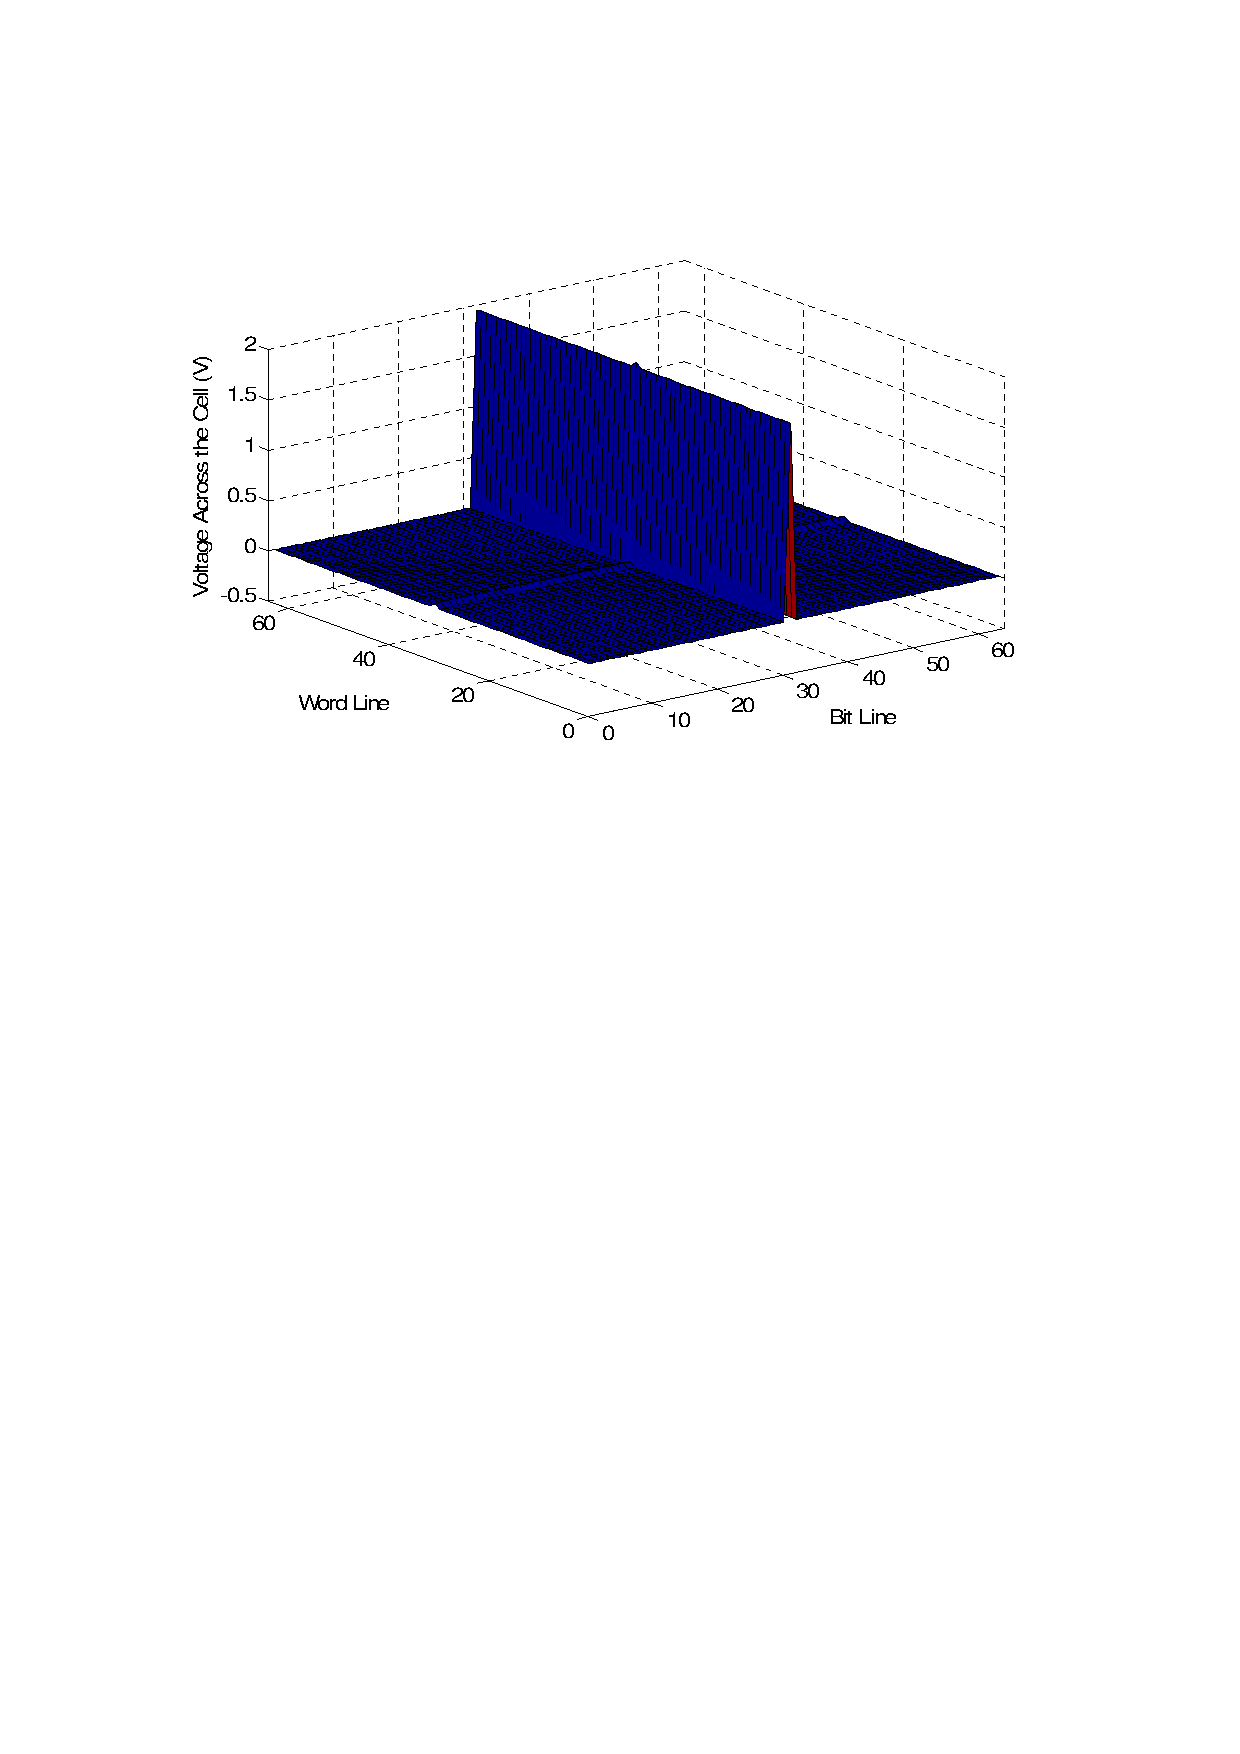
\includegraphics[width=0.4\textwidth]{./figures/FWFB2.pdf}\\
  \caption{Write Disturbance for FWFB Schemes. ( $V_{W32} = 2V$, $V_{B32} = 0V$. $R_{x,32}$ at HRS, others at LRS.) }\label{fig:FWFR}
\end{figure}

The write failure results from the voltage drop at the interconnect wires
along the word line and bit line It has been shown that, for one bit per
access write operation, the worst case of voltage drop is:
\begin{equation}
\left\{
\begin{array}{l}
R_{i,j}=R_{on}\\
V_{WM}=V_W(W)\\
V_{BN}=V_B(W).
\end{array} \right.
\end{equation}
In order to avoid the \textbf{write failure} and successful program the
selected ReRAM cell, the driven voltage should be increased to a higher
level, making sure the voltage across the cell exceed the threshold
voltage at the worst case. Figure.~\ref{fig:worst_v} shows the lower bound
of the driven voltage for different size of cross-point array. The minimum
word/bit line voltage increases from 2.01 V for a $8 \times 8$ array to
4.47 V for a $128 \times 128$ cross-point array. Besides, for a given
memory capability, the cross-point can be organized with different number
of word line and bit line. For example, a 4K bits cross-point array can be
implemented either by a $64 \times 64$ array or by a $32 \times 128$
array. In the latter case, the voltage drops along the word line and bit
line are different with each other. Therefore, Figure.~\ref{fig:shape}
exams the voltage requirement for different array organization. The
results show that from the reliability point of view, the cross-point
array with same numbers of word line and bit line is the best choice.

%Clearly, the magnitude of the voltage drop increases with the array size and the resistance of interconnect wires.

\begin{figure}%[!hb]
\centering
  % Requires \usepackage{graphicx}
  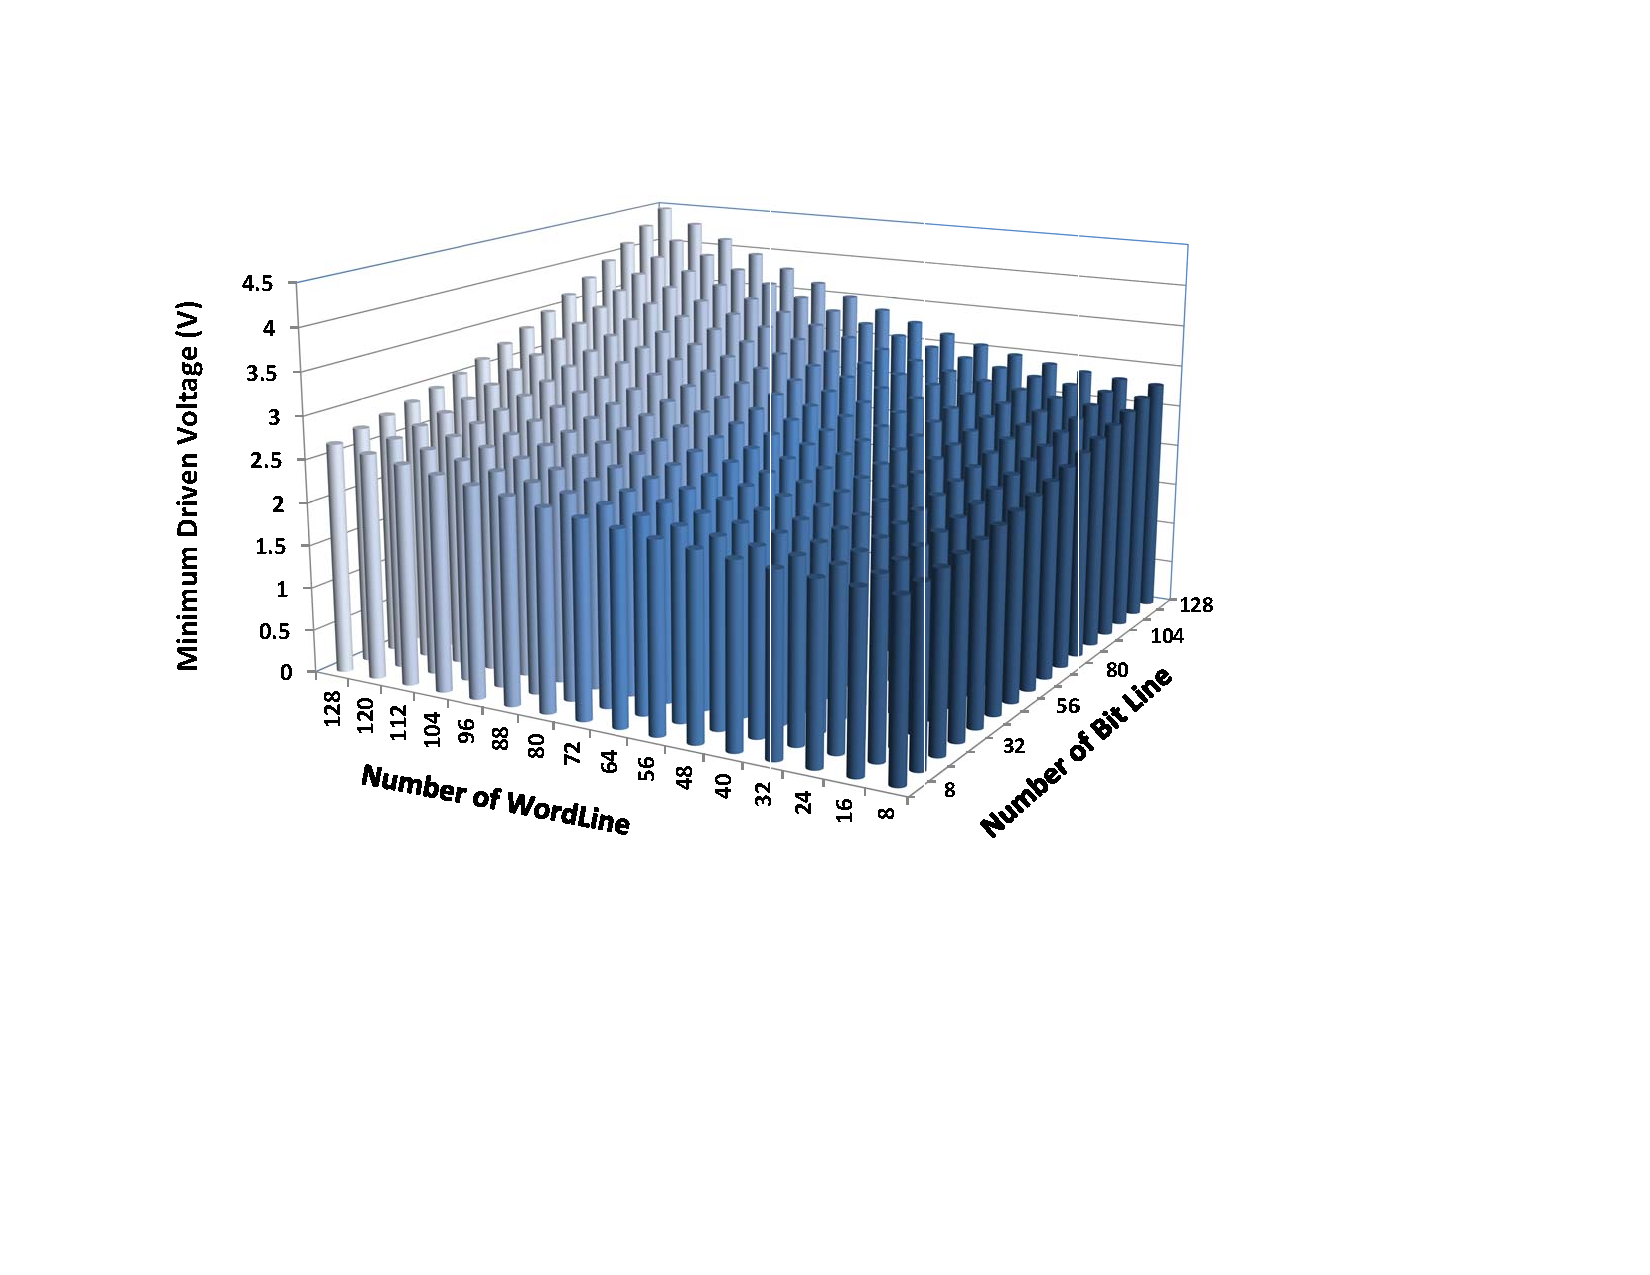
\includegraphics[width=0.4\textwidth]{./figures/worst_v2.pdf}\\
  \caption{Write Voltage Requirement (Threshold Voltage = 2V). }\label{fig:worst_v}
\end{figure}


\begin{figure}%[!t]
\centering
  % Requires \usepackage{graphicx}
  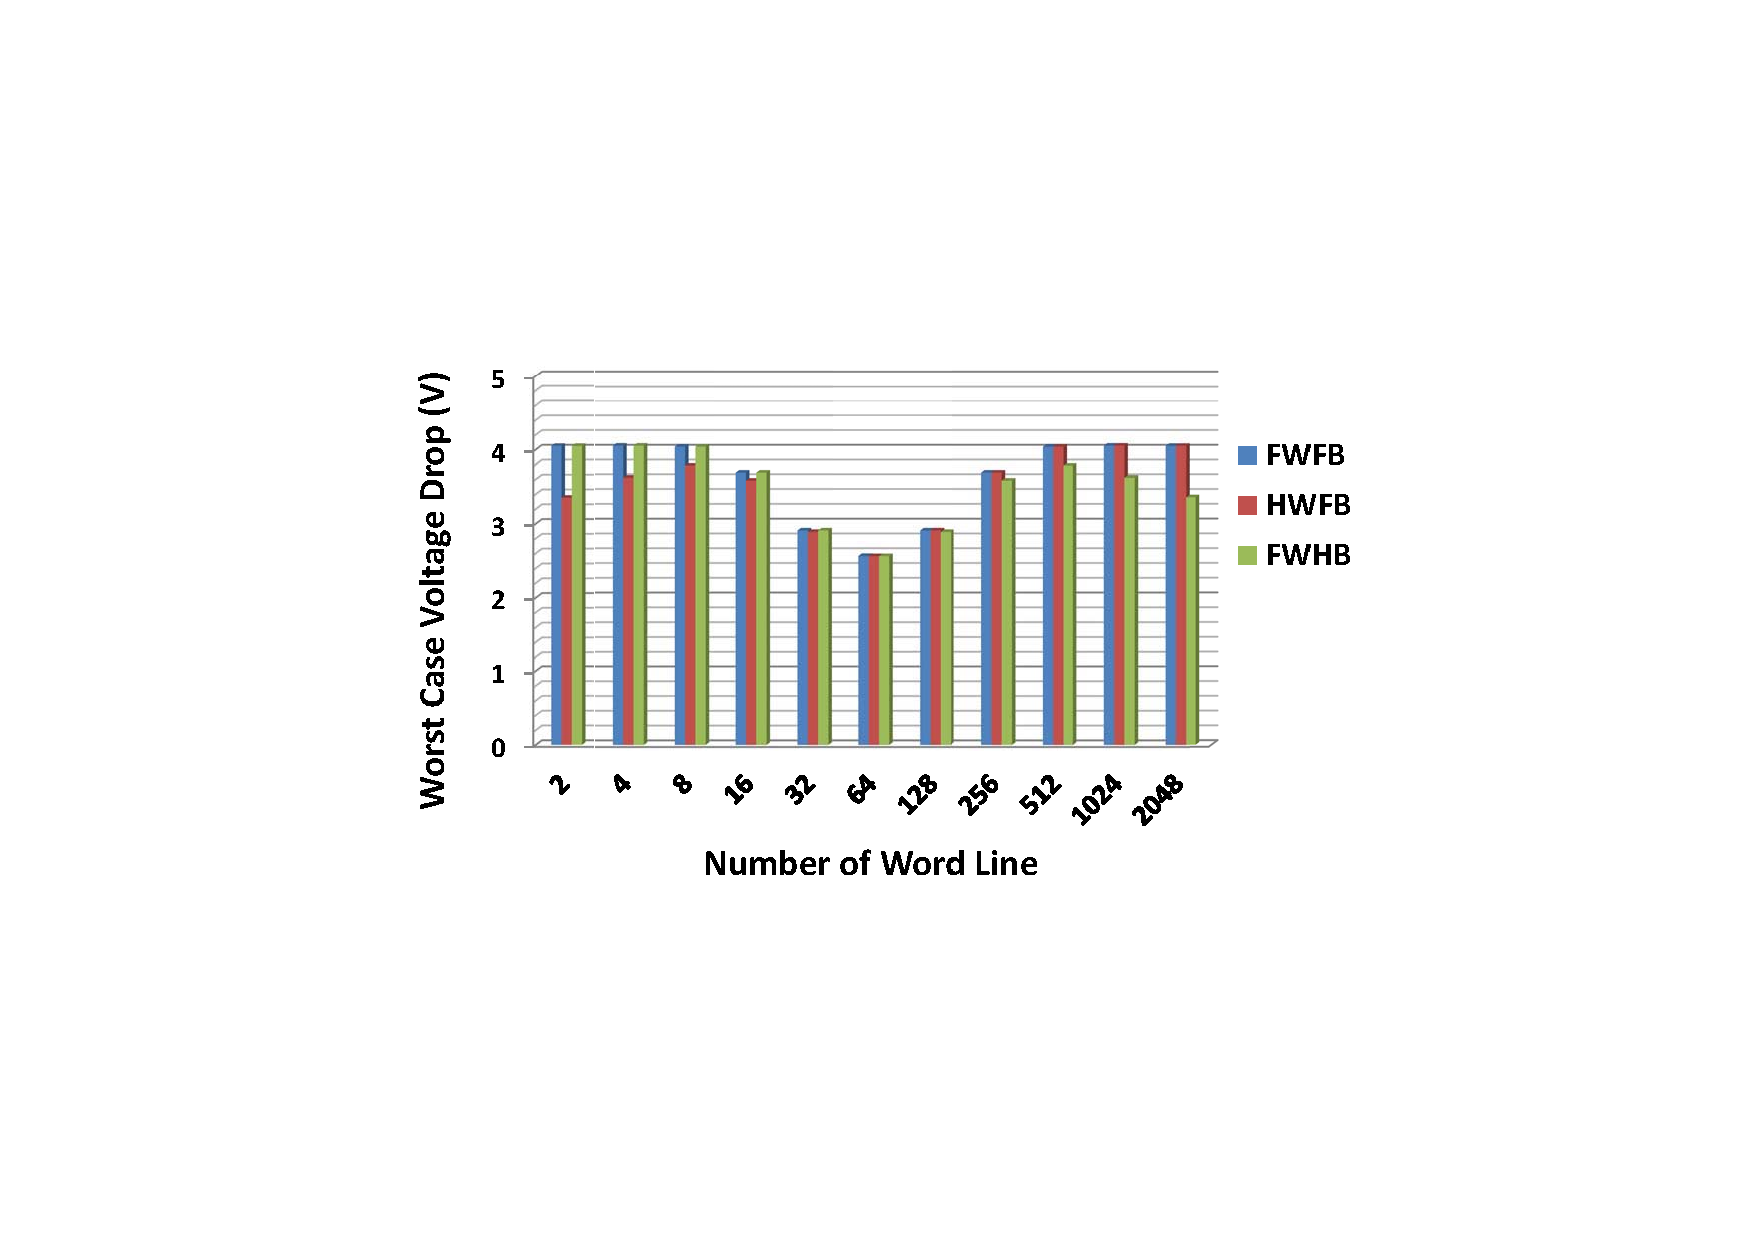
\includegraphics[width=0.45\textwidth]{./figures/shape2.pdf}\\
  \caption{Write Voltage Requirement with Different Memory Shape. (Array Capacity = 4Kbits, Activated Word Line Voltage = 2V, Activated Bit Line Voltage = 0V.)}\label{fig:shape}
\end{figure}

However, in the other hand, the increasing of the driven voltage also
increases the voltage applied at the unselected cell. Therefore, a
\textbf{write disturbance} will occur when the voltage applied at the
unselected cell exceeds the threshold voltage for SET or RESET operation.
Figure.~\ref{fig:half} shows the worst case (maximum) voltage applied at
unselected cells with the minimum driven voltage shown in
Figure~\ref{fig:worst_v}. Since the threshold voltage of the cell is 2V,
all of the word/bit line combinations at the region with worst case
voltage more than 2V are unreliable and can not avoid write failure and
write disturbance at the same time. Thus, Figure.~\ref{fig:half} provides
the hard constraint of array size, and all of the following energy and
area tradeoffs should be bounded by this constraint.

\begin{figure}%[!t]
\centering
  % Requires \usepackage{graphicx}
  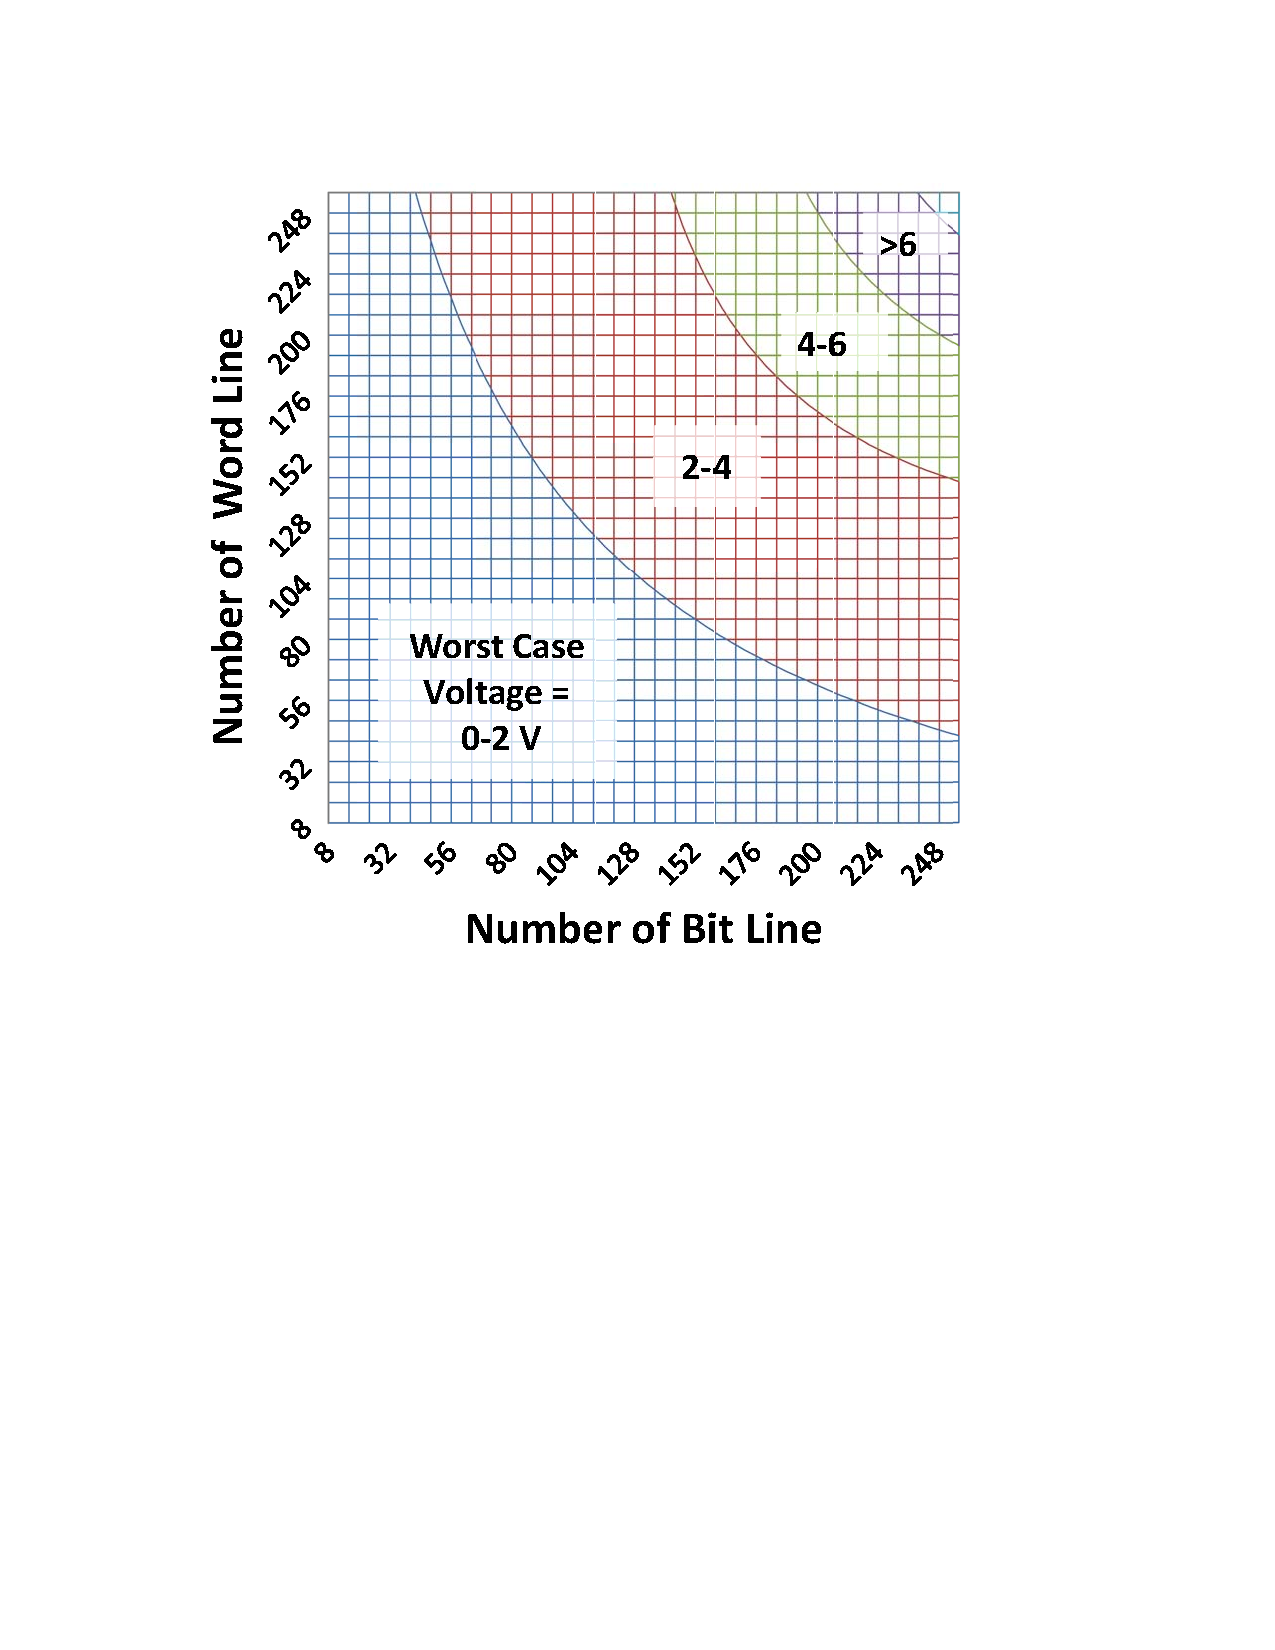
\includegraphics[width=0.3\textwidth]{./figures/Theoretical_bound.pdf}\\
  \caption{The }\label{fig:half}
\end{figure}



\vspace{10pt} \textbf{Energy Consumption of Write Operation.} \vspace{8pt}

The energy consumption of a write operation for a cross-point array can be calculated as:
\begin{equation}
E_{write} = E_{select} + E_{unselect} + E_{halfselect} + E_{line},
\end{equation}
where the $E_{select}$ is the energy consumed to change the state of the
selected cell, the $E_{unselect}$ and $E_{halfselect}$ are the undesired energy wasted at the half selected and unselected cells. The energy consumed by the interconnect lines are represented by $E_{line}$. Figure.~\ref{fig:energy} shows each part's energy consumption for the cross-point array. Firstly, the $E_{line}$ and $E_{halfselect}$ take a large amount of the total energy consumption. Besides, the energy wasted during the write operation is much larger than the energy required to program the ReRAM cell. For example, the energy consumption for writing a $128{\times}128$ array is more than 1000 times larger than the $8{\times}8$ array. We also notice that, since the impact of sneak paths for floating schemes (FWHB and HWFB) is much serious, the energy consumed at unselected cells for the floating schemes are much larger than the half-biased scheme. Therefore, the total energy consumptions for FWHB and HWFB schemes are at least 10\% larger than that of HWHB scheme.


\begin{figure}%[!t]
\centering
  % Requires \usepackage{graphicx}
  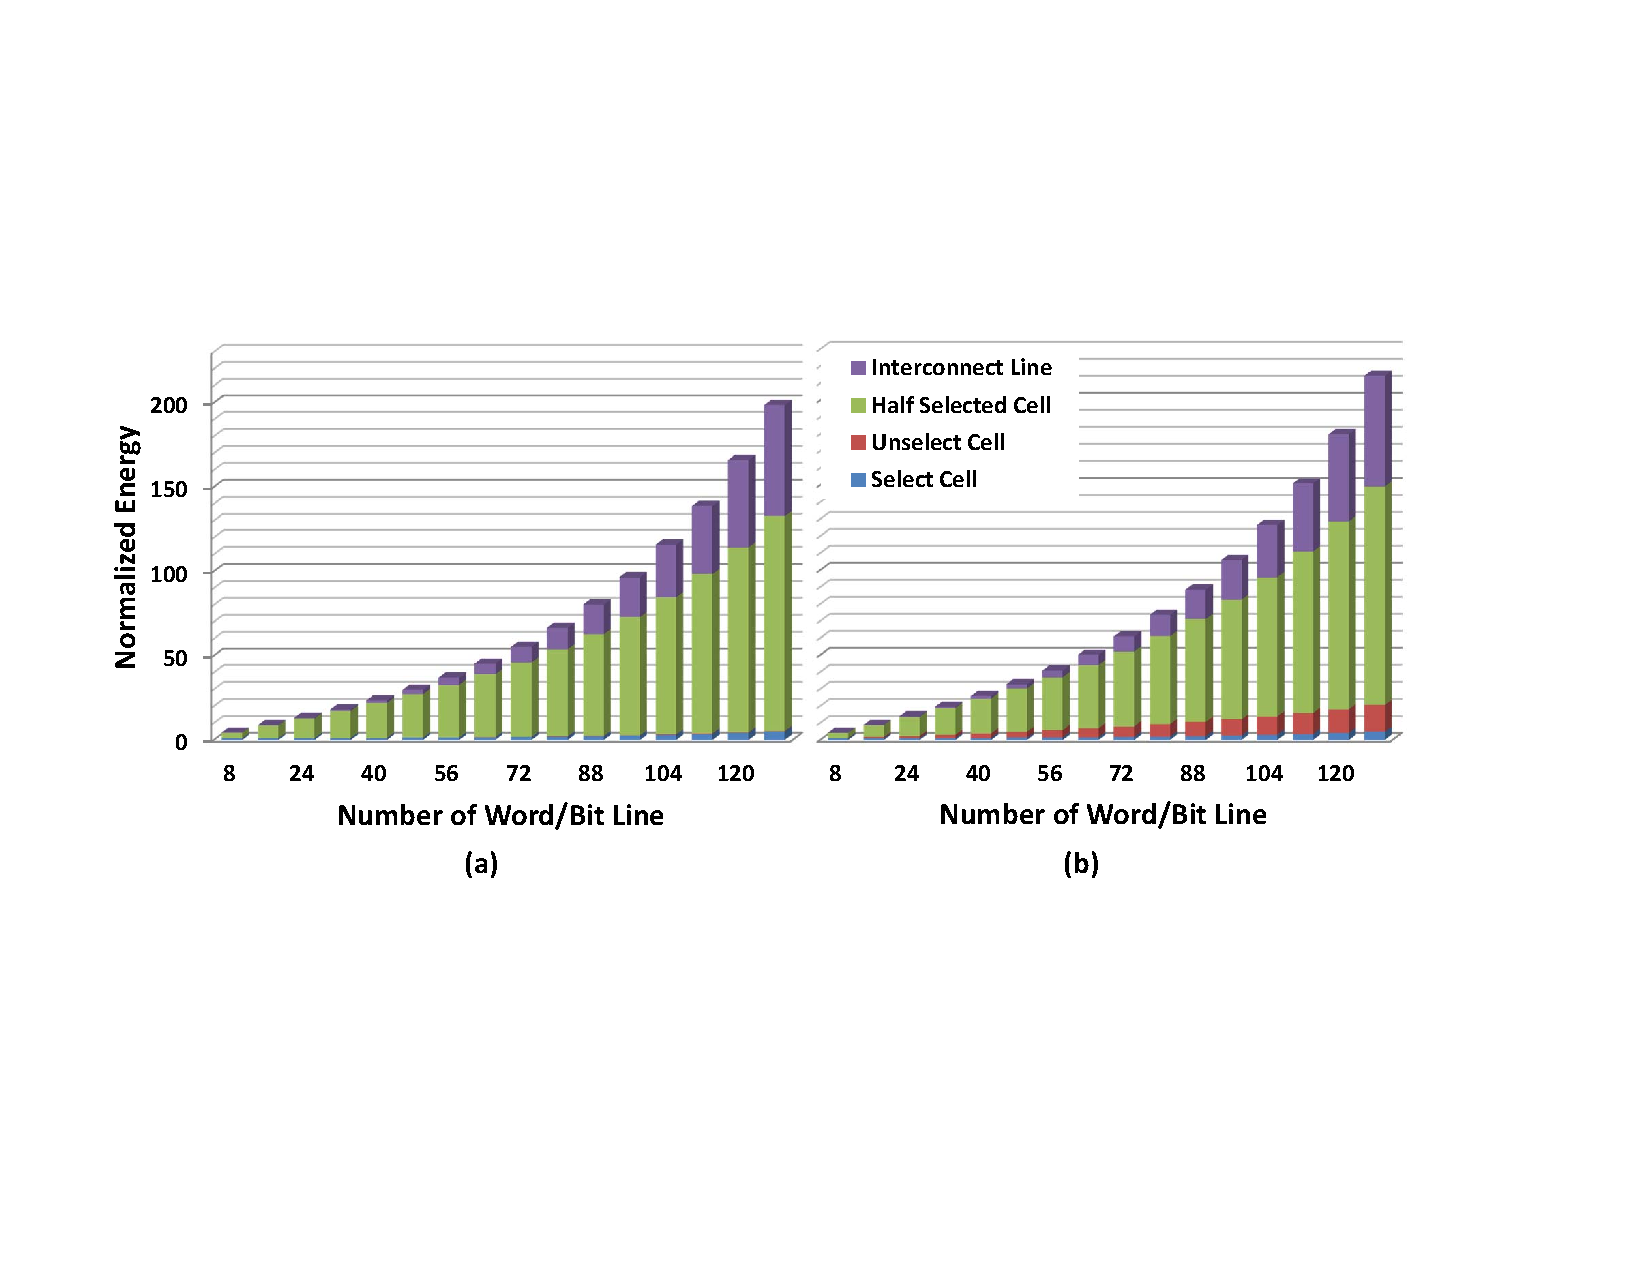
\includegraphics[width=0.45\textwidth]{./figures/energy4.pdf}\\
  \caption{The Normalized Energy Consumption. (a): HWHB scheme (b): FWHB and HWFB schemes.}\label{fig:energy}
\end{figure}

\vspace{10pt} \textbf{Area cost of Write Operation.} \vspace{8pt}

The write operation requires $m+n$ voltage driver to provide enough current for each word line and bit line for a $m{\times}n$ array.
Therefore, the average number of ReRAM cells per voltage driver can be
calculated as $mn/(m+n)$. By given an array capacity $C_{array}$, it is
easy to find that the optimal array organization can be achieved when
$m=n=\sqrt{C_{array}}$ and the maximum number of cells per voltage driver
is: $\sqrt{C_{array}}/2$. However, the area overhead of the voltage driver also related to the driven current. Figure.~\ref{fig:w_current} shows the required driven current for different size of ReRAM array. According to the current requirement, the area of the voltage driver can be directly calculated, which will be shown in the following discussion.

\begin{figure}%[!t]
\centering
  % Requires \usepackage{graphicx}
  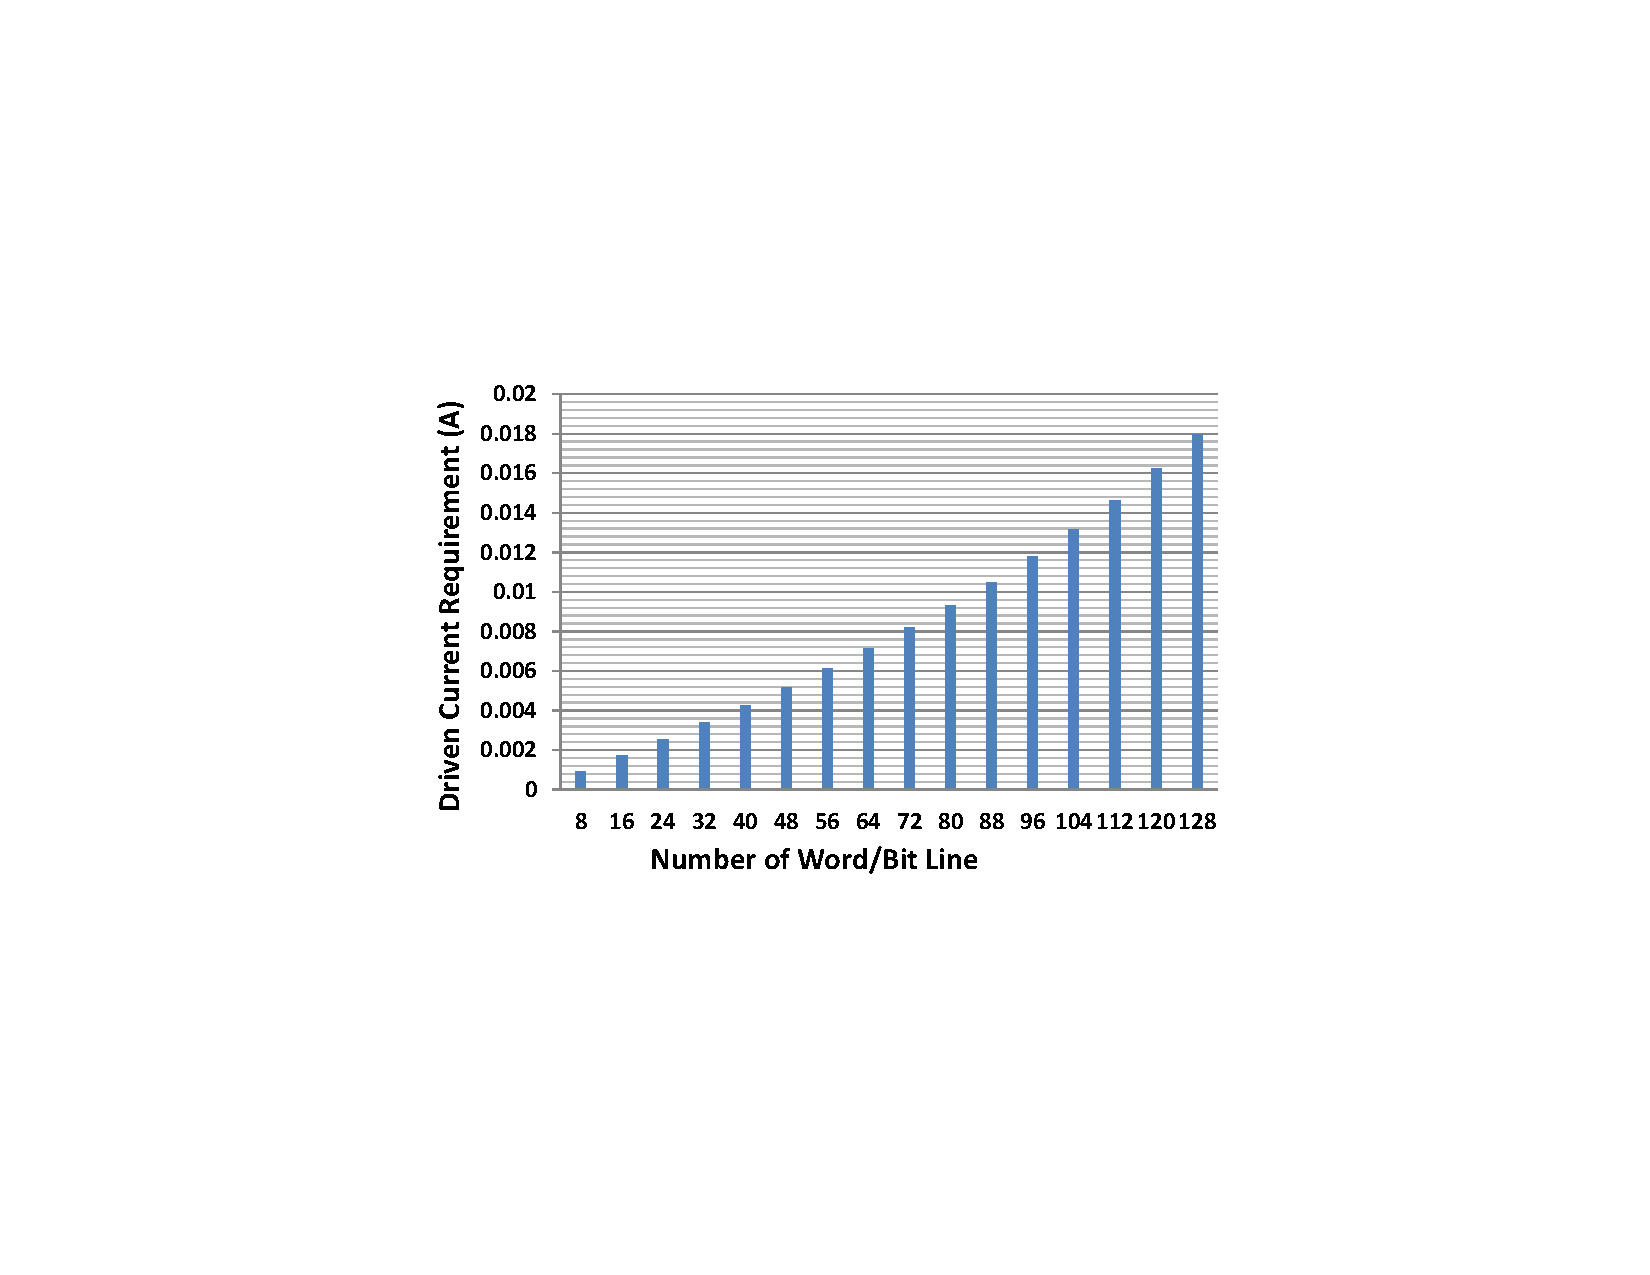
\includegraphics[width=0.4\textwidth]{./figures/w_current2.pdf}\\
  \caption{The }\label{fig:w_current}
\end{figure}

\vspace{10pt} \textbf{Discussion on Multi-Bits Write Operation.} \vspace{8pt}

So far, we only discuss the one bit per access write operation. At this section, the difference between one bit per access and one word line per are discussed. Firstly, writing a word line at the same time will worsen the voltage drop along the word line. Therefore, as shown in Figure.~\ref{fig:reliable_region}, the reliable size of the cross-point array will be further reduced. The maximum array size reduces from $116{\times}116$ to $100{\times}100$ for HWFB and HWFB schemes. For the energy consumption point of view, the one word line write operation is more efficient.


\begin{figure}%[!t]
\centering
  % Requires \usepackage{graphicx}
  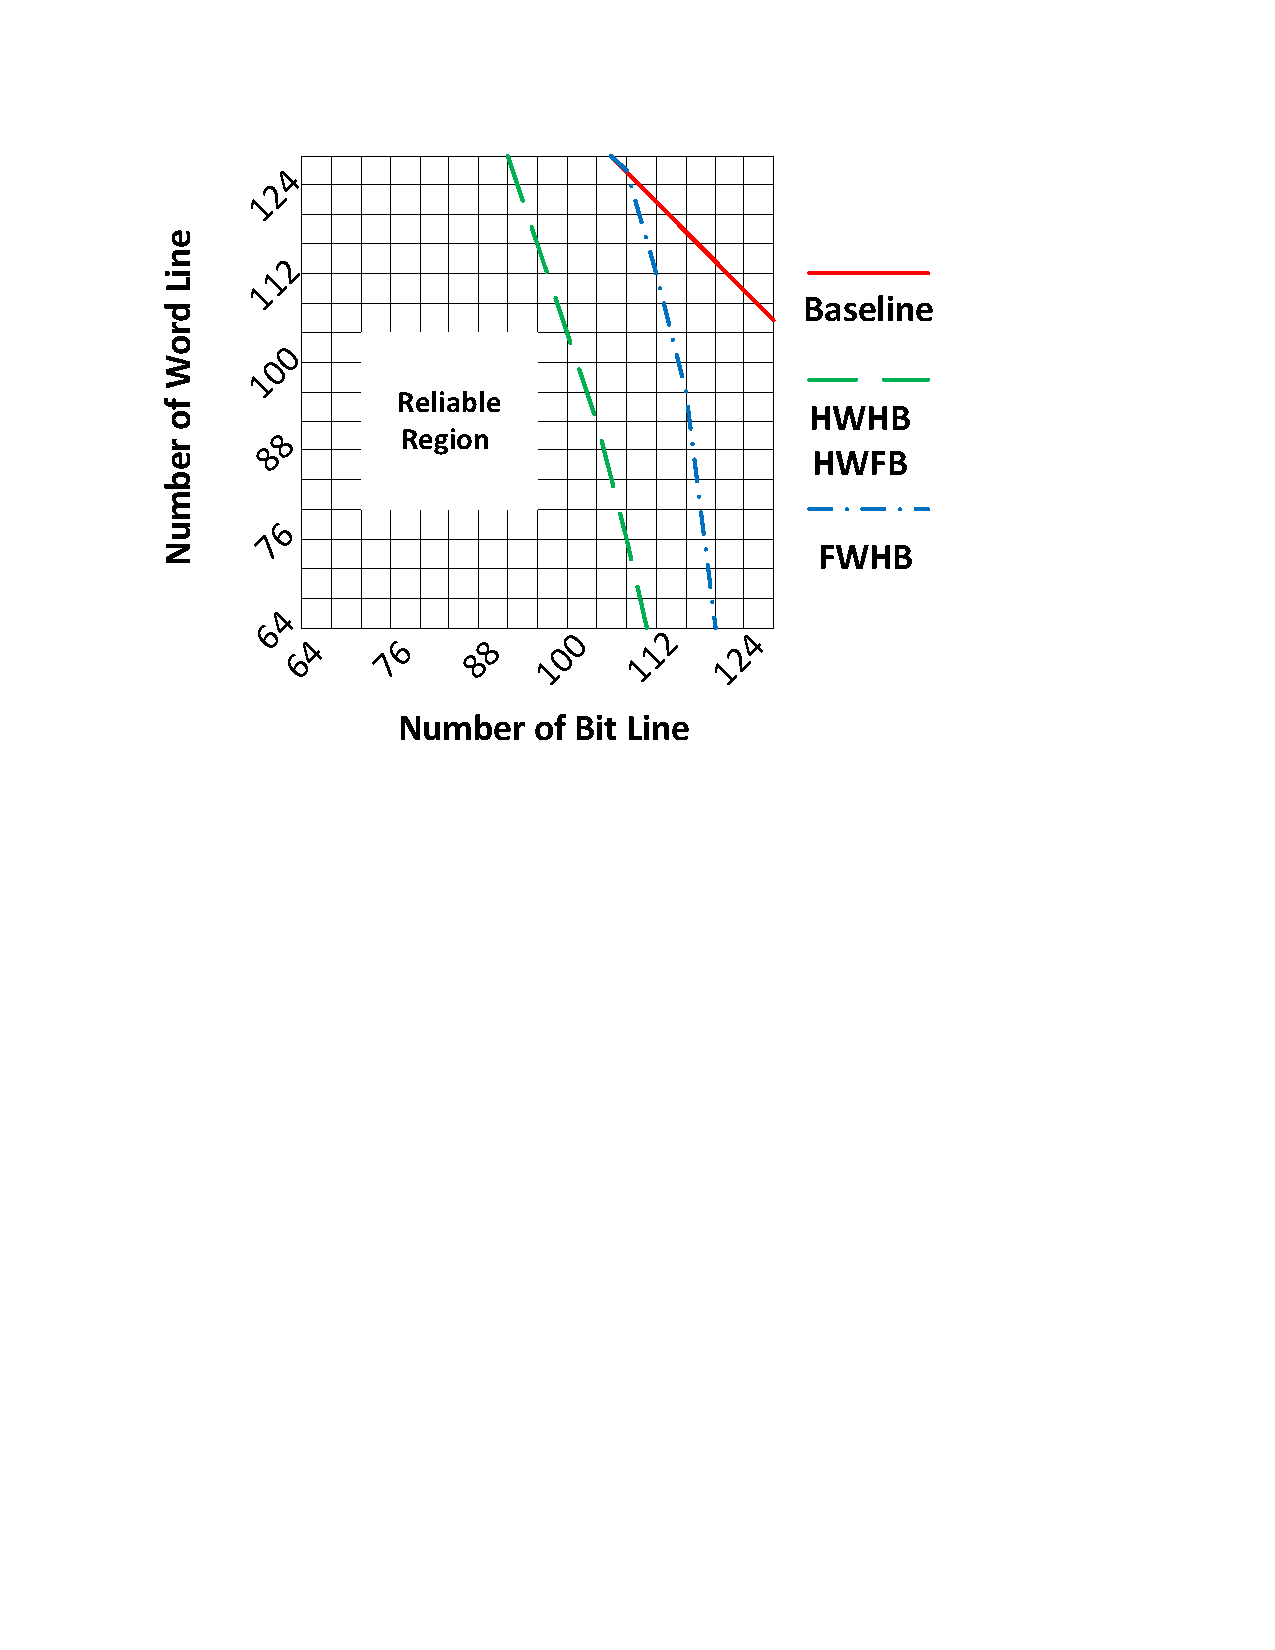
\includegraphics[width=0.4\textwidth]{./figures/multiwrite.pdf}\\
  \caption{The Array Size Requirement for the Cross-Point Array with Different Write Schemes. (Baseline: one bit per access. HWHB, HWFB and FWHB: one word line per access. }\label{fig:reliable_region}
\end{figure}

In order to fairly compared the energy consumption, Figure.~\ref{fig:multi_energy} shows the average energy for writing one bit during the multi-bit write operation. For example, in order to write a word line with size of 128, the average energy can be calculated as:
$E_{ave}=E_{total}/128/2$. The energy shown in Figure.~\ref{fig:multi_energy} is normalized to the same unit as Figure.~\ref{fig:energy}. The results show that for large size of the cross point array, the multi-bit write operation is much more energy efficiency. The reason is that the energy wasted at the unselected and half-selected cells are shared by multi bits and the average energy for one each bit is therefore reduced. However, even the multi-bit write operation has the advantage on energy consumption, the driven current requirement for each word line also increases. As shown in Figure.~\ref{fig:multi_I}, although the maximum driven current for bit line is almost the same as one bit writing, the drive capability for wold line is doubled for multi-bit writing. Since the area of the voltage driver increases proportional with its driven capability, the area overhead for multi-bit writing is about 50\% larger than one bit writing.


\begin{figure}%[!t]
\centering
  % Requires \usepackage{graphicx}
  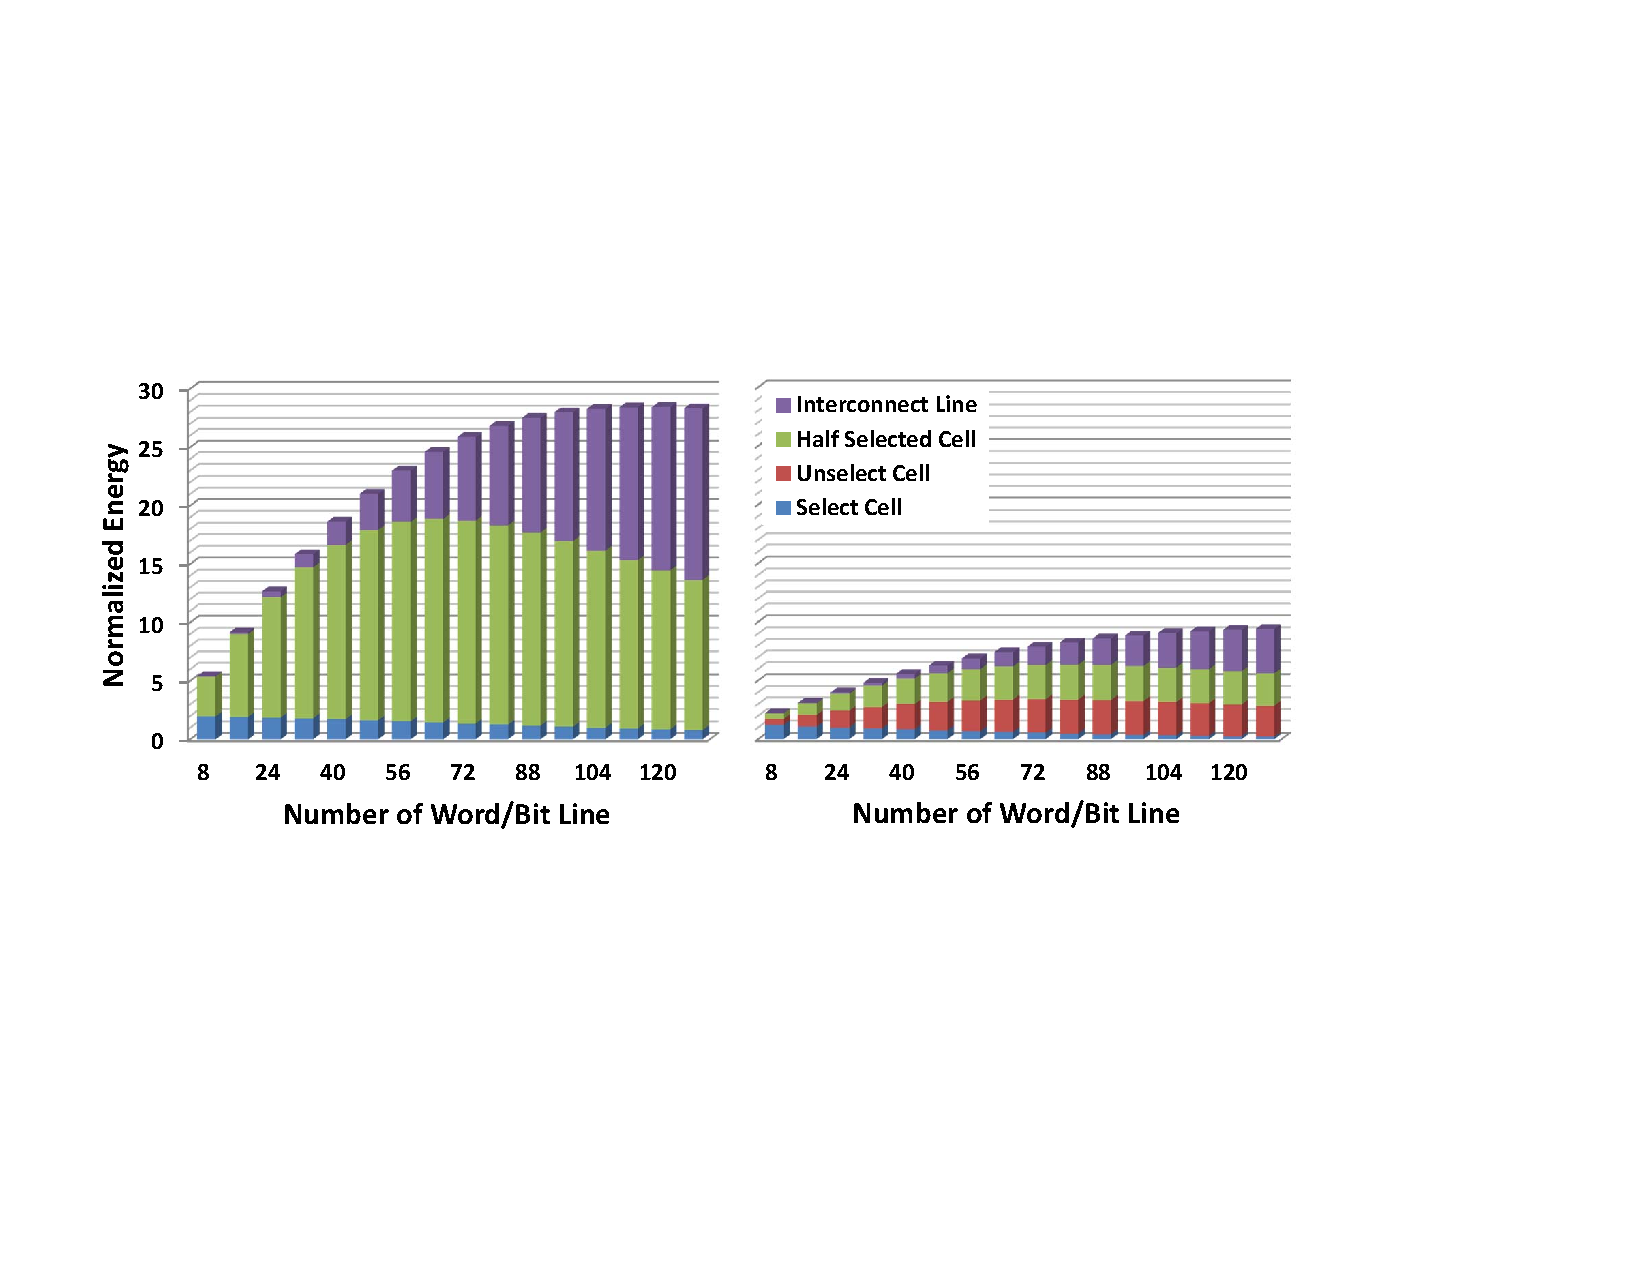
\includegraphics[width=0.45\textwidth]{./figures/multi_energy2.pdf}\\
  \caption{The Normalized Energy Consumption per Bit for Multi-Bits Write Operation. (a): HWHB and  FWHB schemes (b): HWFB scheme. }\label{fig:multi_energy}
\end{figure}


\begin{figure}%[!t]
\centering
  % Requires \usepackage{graphicx}
  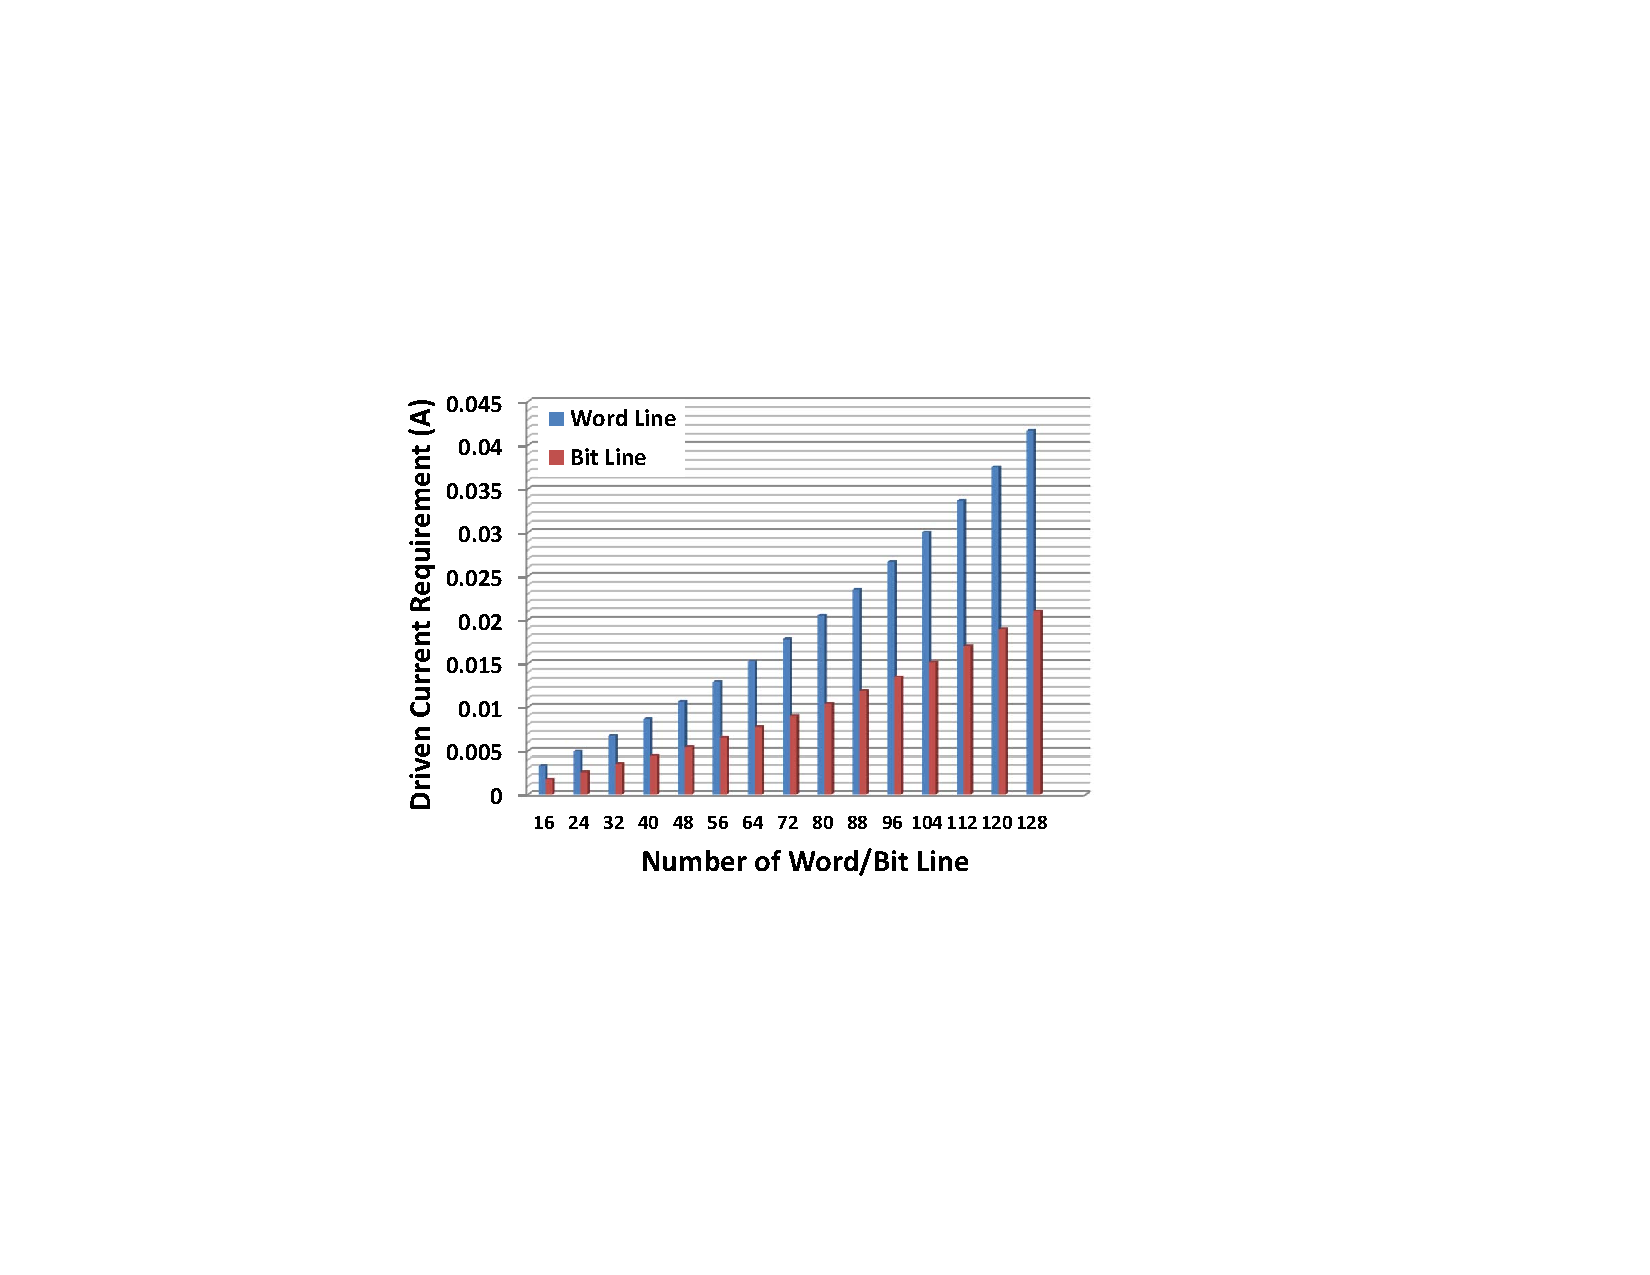
\includegraphics[width=0.4\textwidth]{./figures/multi_I2.pdf}\\
  \caption{The }\label{fig:multi_I}
\end{figure}

\vspace{10pt} \textbf{Non-linearity of the ReRAM Cell.} \vspace{8pt}

One of the most distinct feature of ReRAM is it non-linearity. Take the memristor based ReRAM for example, the non-linearity can be described as: the resistance of the memristor cell is not constant but varies with the applied voltage. The non-linearity coefficient is defined as:
$K_r(p,V) = p \times R(V/p)/R(V)$, where $R(V/p)$ and $R(V)$ are equivalent resistance of the memristor biased at $V/p$ and $V$~\cite{memristor:Cong}. Normally, the $K_r(p,V)$ value for memristor based ReRAM is larger than 5, meaning that the resistance of half-biased  cell is 10 times larger than full-biased cell. Clearly, the ReRAM cell with larger non-linearity coefficient is more suitable to be employed as the memory cell since the current in the sneak path will be significantly reduced. Besides, the increased resistance at half-selected and unselected cell can also mitigate the voltage drop along the activated word line and bit line. Figure ~\ref{fig:non_linear} shows the influence of different non-linearity coefficients on the array size requirements. Due to the space limitation, only the results for one bit writing with HWHB scheme are shown. In this figure, the maximum array size increases from $112 \times 112$ to $340 \times 340$ when the non-linearity coefficient $K_r$ increases to 10.

\begin{figure}%[!t]
\centering
  % Requires \usepackage{graphicx}
  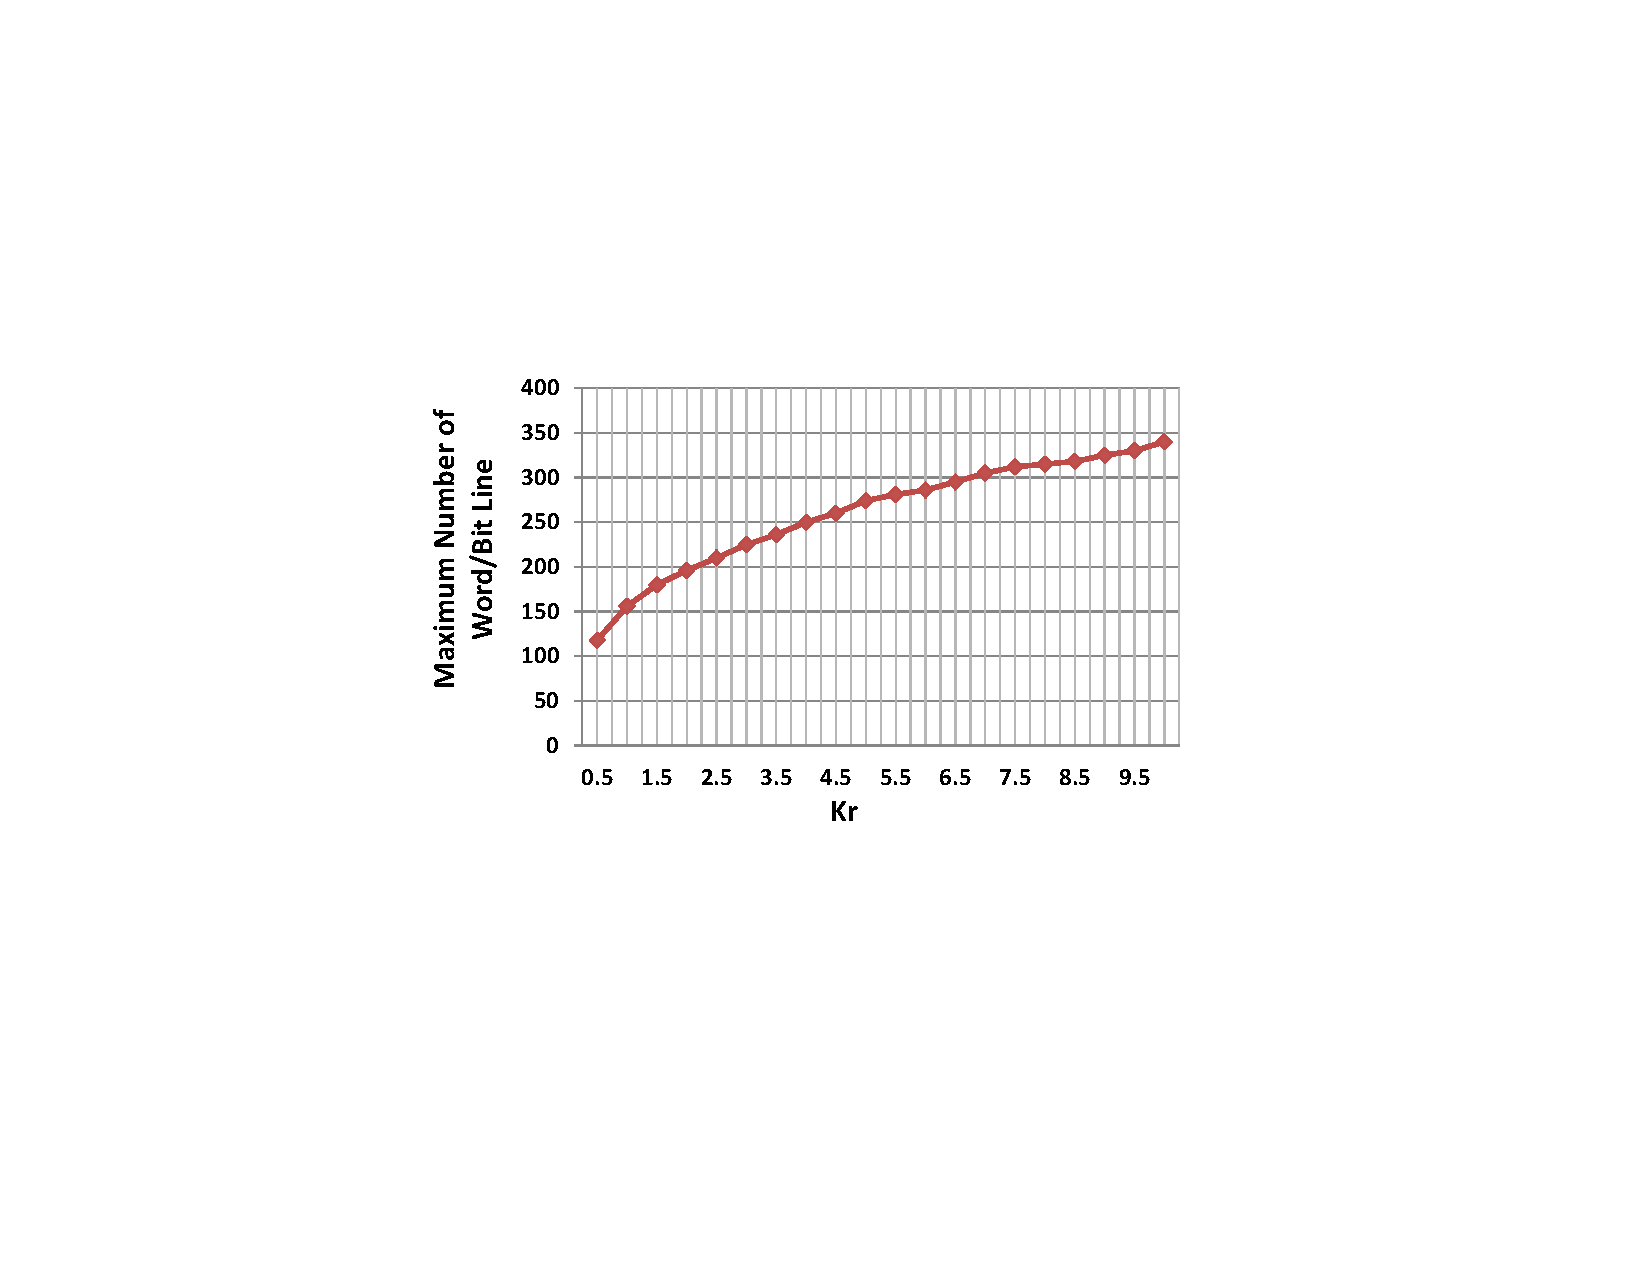
\includegraphics[width=0.4\textwidth]{./figures/non_linear}\\
  \caption{The Maximum Array Size with Different Non-linearity}\label{fig:non_linear}
\end{figure}

On the other hand, the non-linearity can also benefit the energy consumption and area overhead as well. Take the $128 \times 128$ array for example.


\begin{figure}%[!t]
\centering
  % Requires \usepackage{graphicx}
  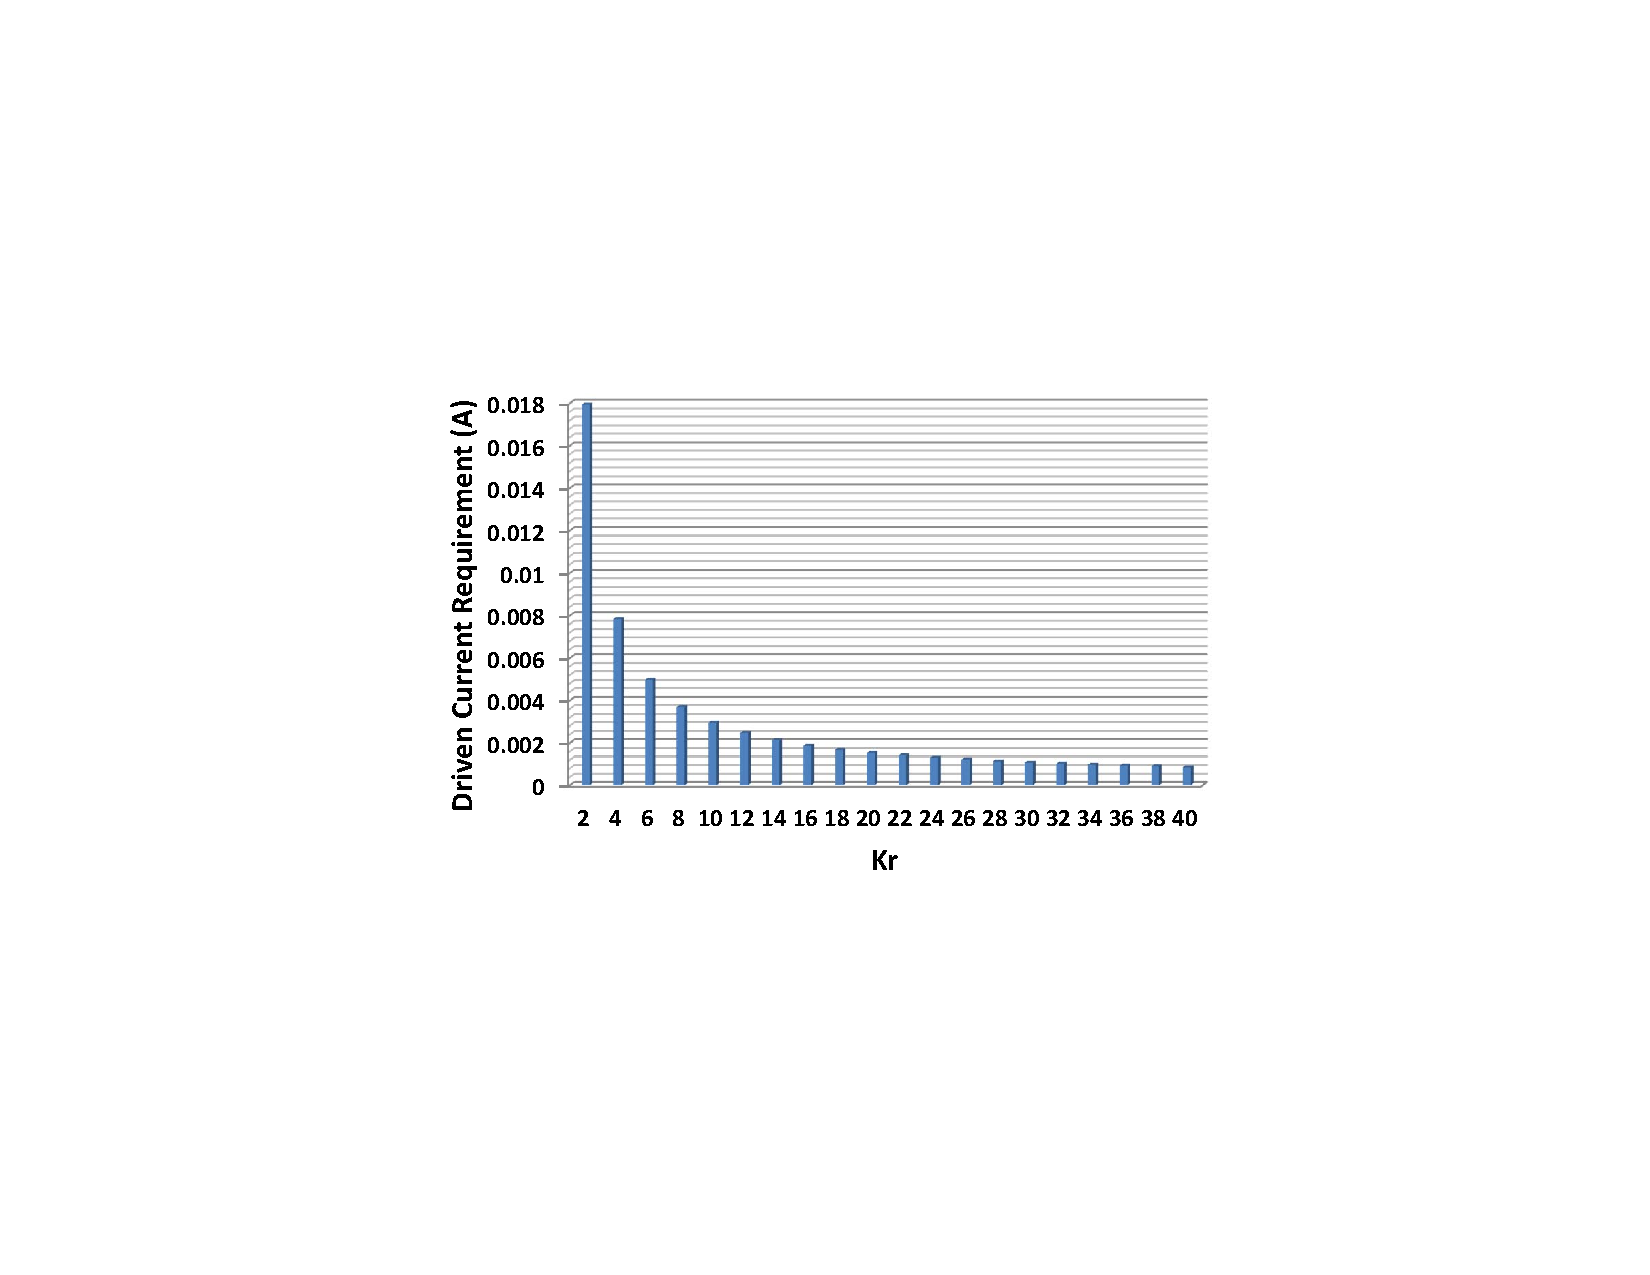
\includegraphics[width=0.4\textwidth]{./figures/non_linear_I.pdf}\\
  \caption{The}\label{fig:non_linear_I}
\end{figure}

\begin{figure}%[!t]
\centering
  % Requires \usepackage{graphicx}
  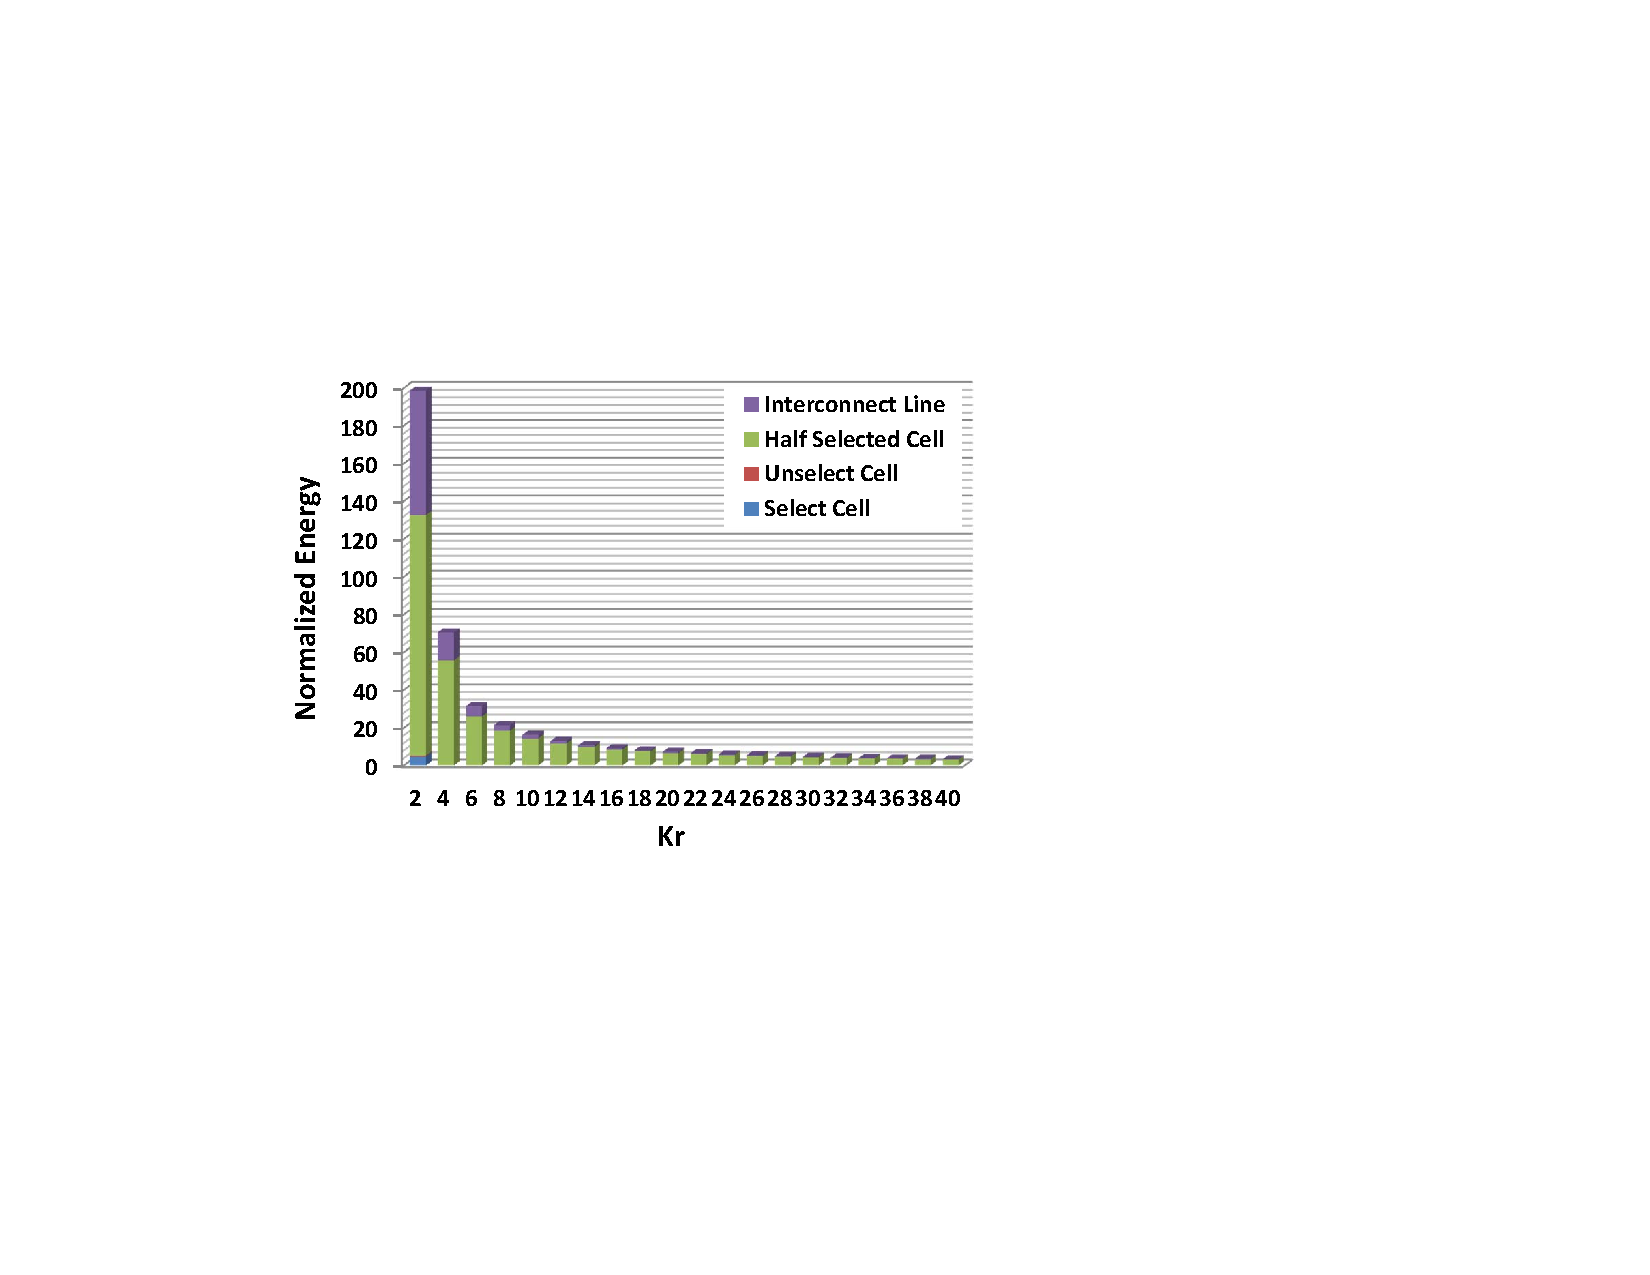
\includegraphics[width=0.4\textwidth]{./figures/non_linear_energy.pdf}\\
  \caption{The}\label{fig:non_linear_energy}
\end{figure}

\begin{figure}%[!t]
\centering
  % Requires \usepackage{graphicx}
  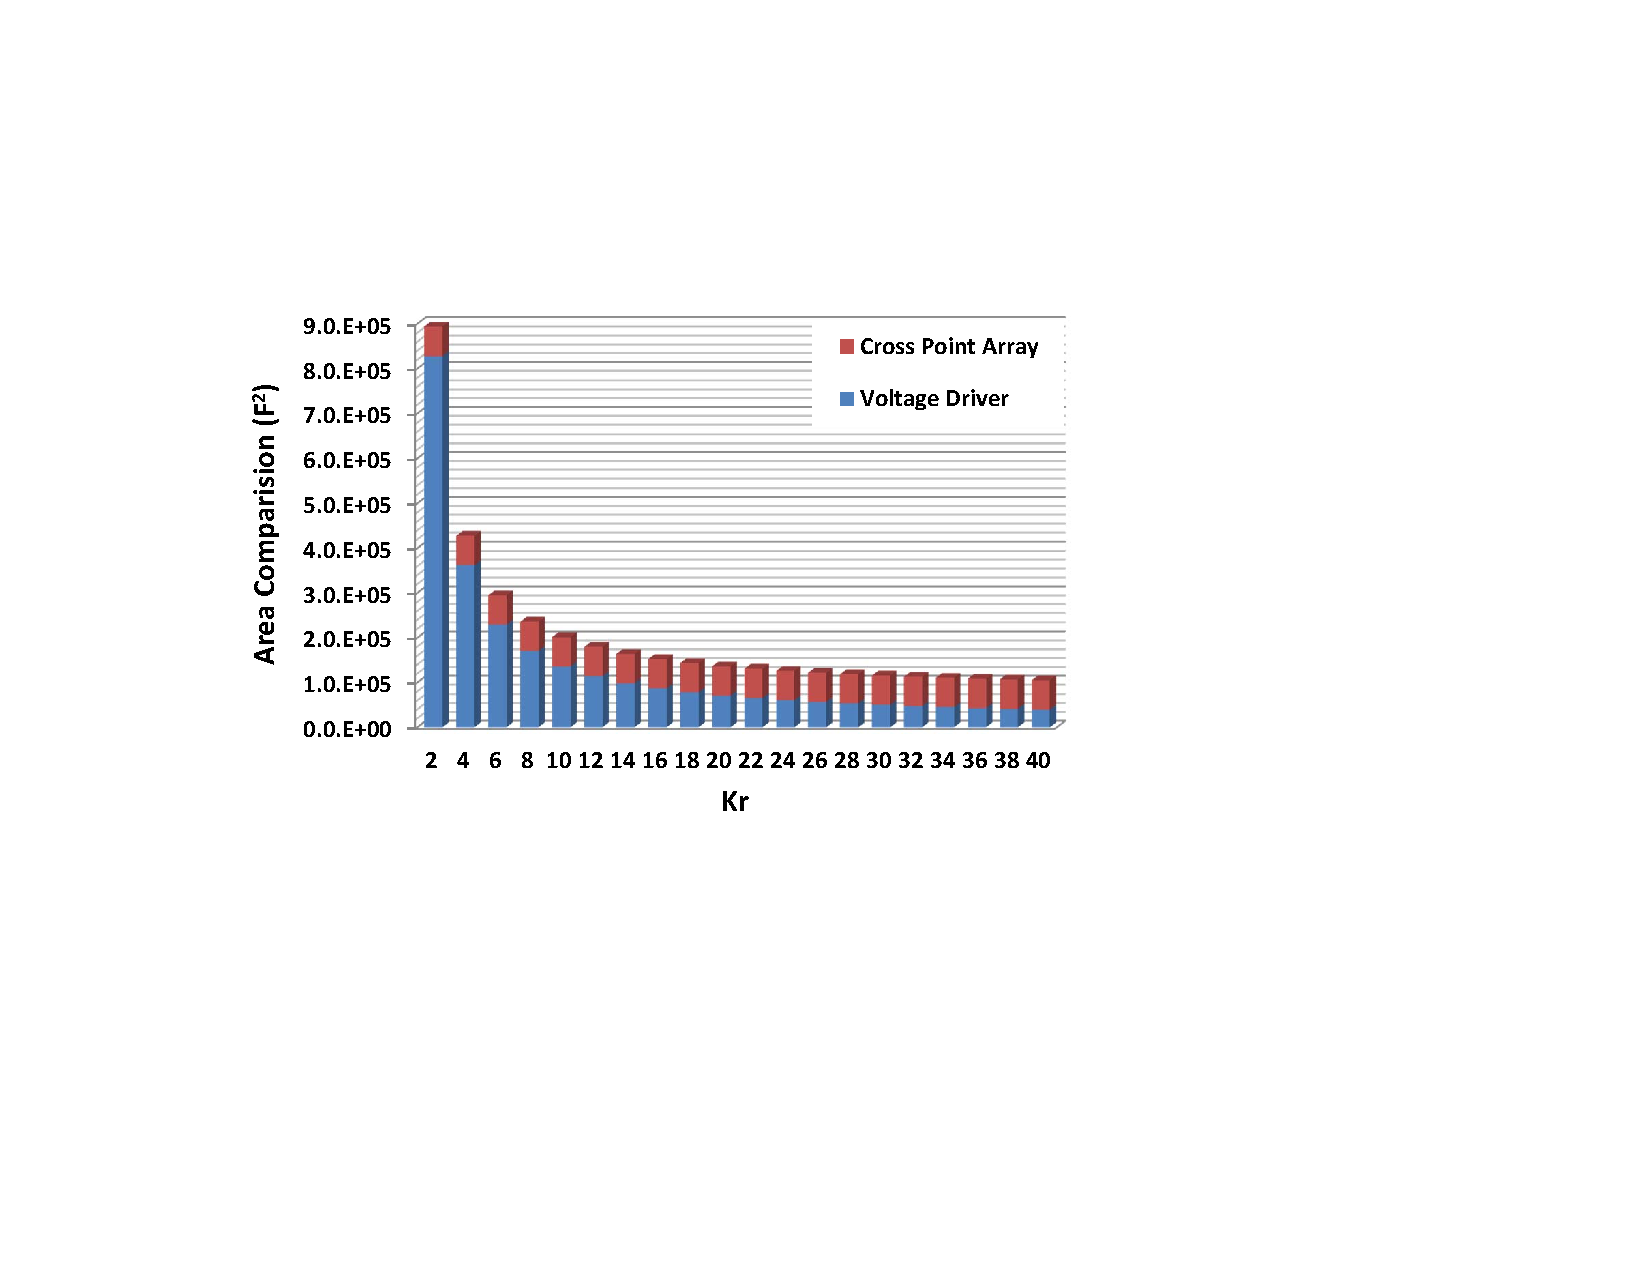
\includegraphics[width=0.4\textwidth]{./figures/non_linear_ara.pdf}\\
  \caption{The}\label{fig:non_linear_ara}
\end{figure}

\begin{figure}%[!t]
\centering
  % Requires \usepackage{graphicx}
  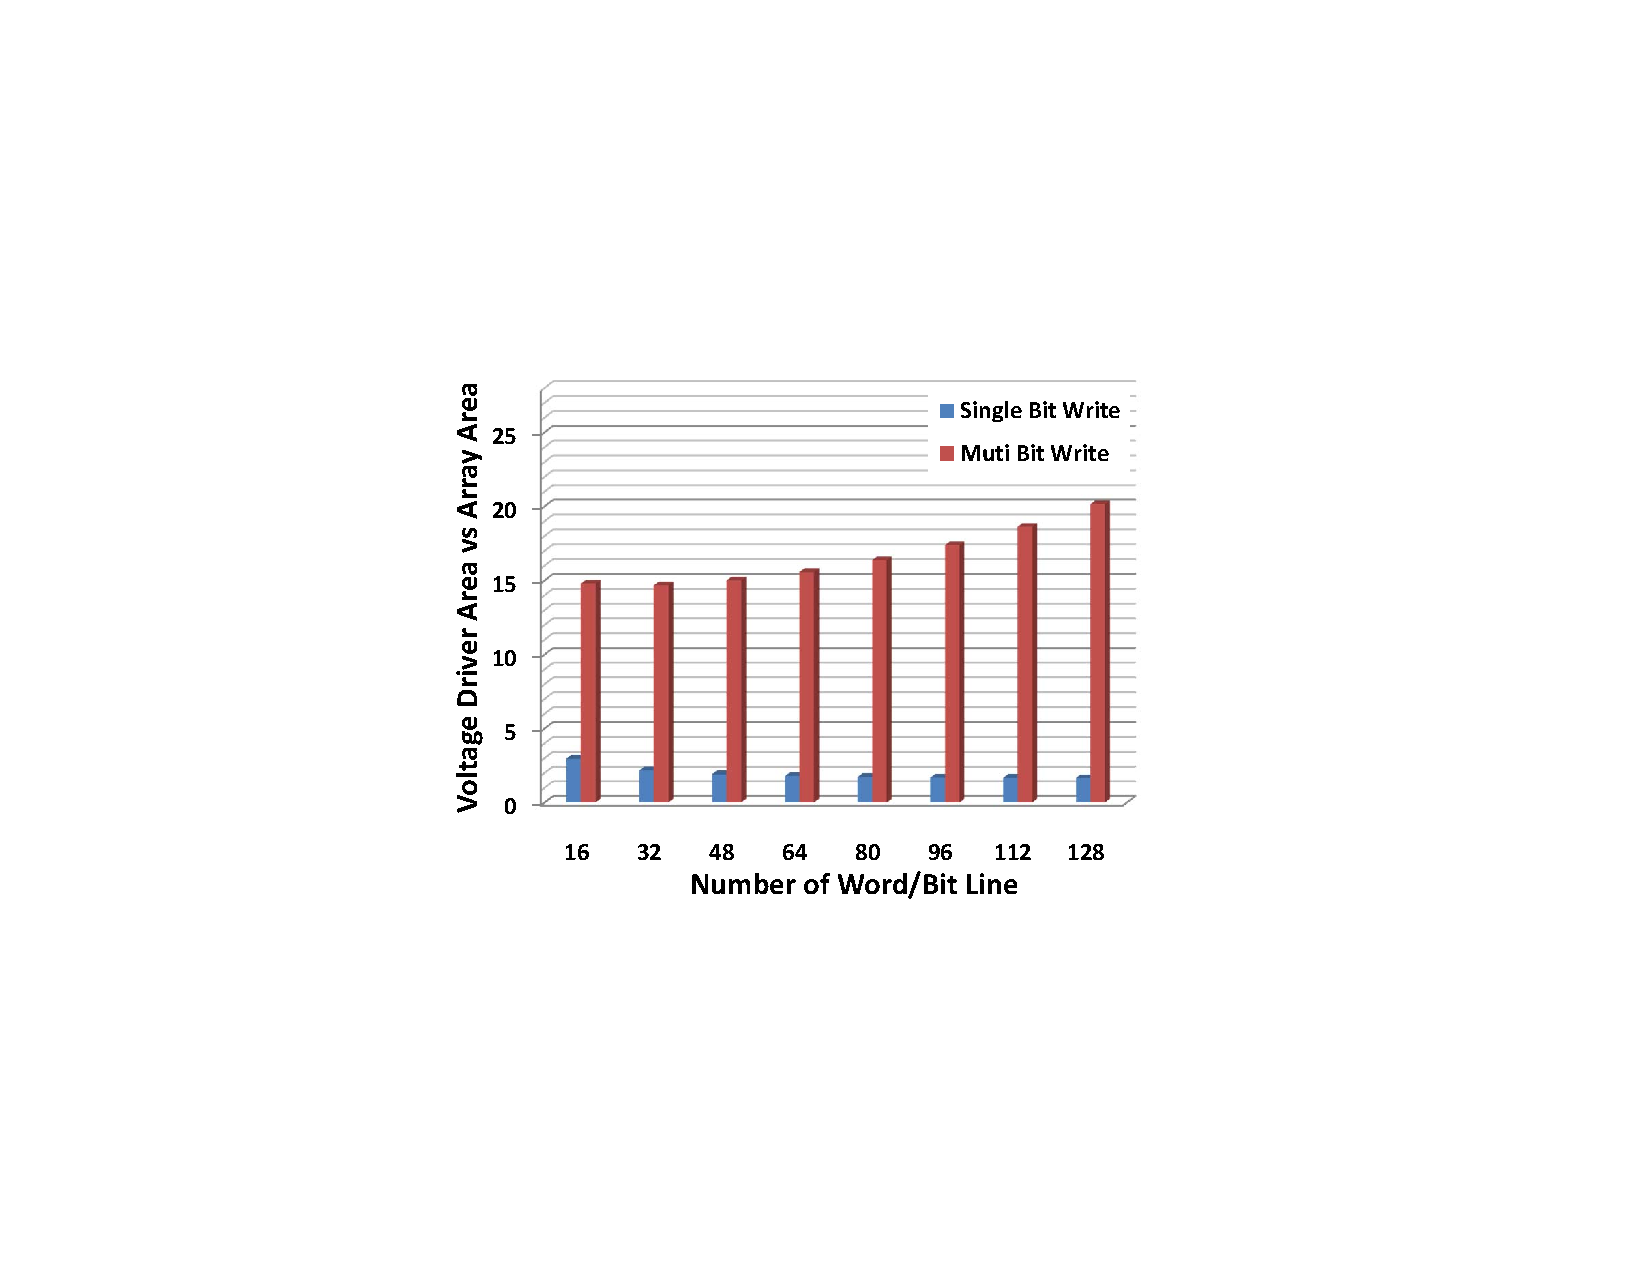
\includegraphics[width=0.4\textwidth]{./figures/Area_kr20.pdf}\\
  \caption{The}\label{fig:Area_kr20}
\end{figure}
\subsection{Read Operation}
The design constraints for read operation can be analyzed by the same way as the write operation, including the reliability, energy consumption and the area overhead. Note that the read voltage/current is much lower than the write voltage, therefore we believe the voltage drivers can always provide enough current for the read operation if they meet the current requirement for write operation. Thus in this section, we only shows the results of reliability issue and read energy. Also, since the difference

The reliability issue of the read operation of the cross bar array are well studied in previous researches.
%\begin{figure}%[!t]
%\centering
%  % Requires \usepackage{graphicx}
%  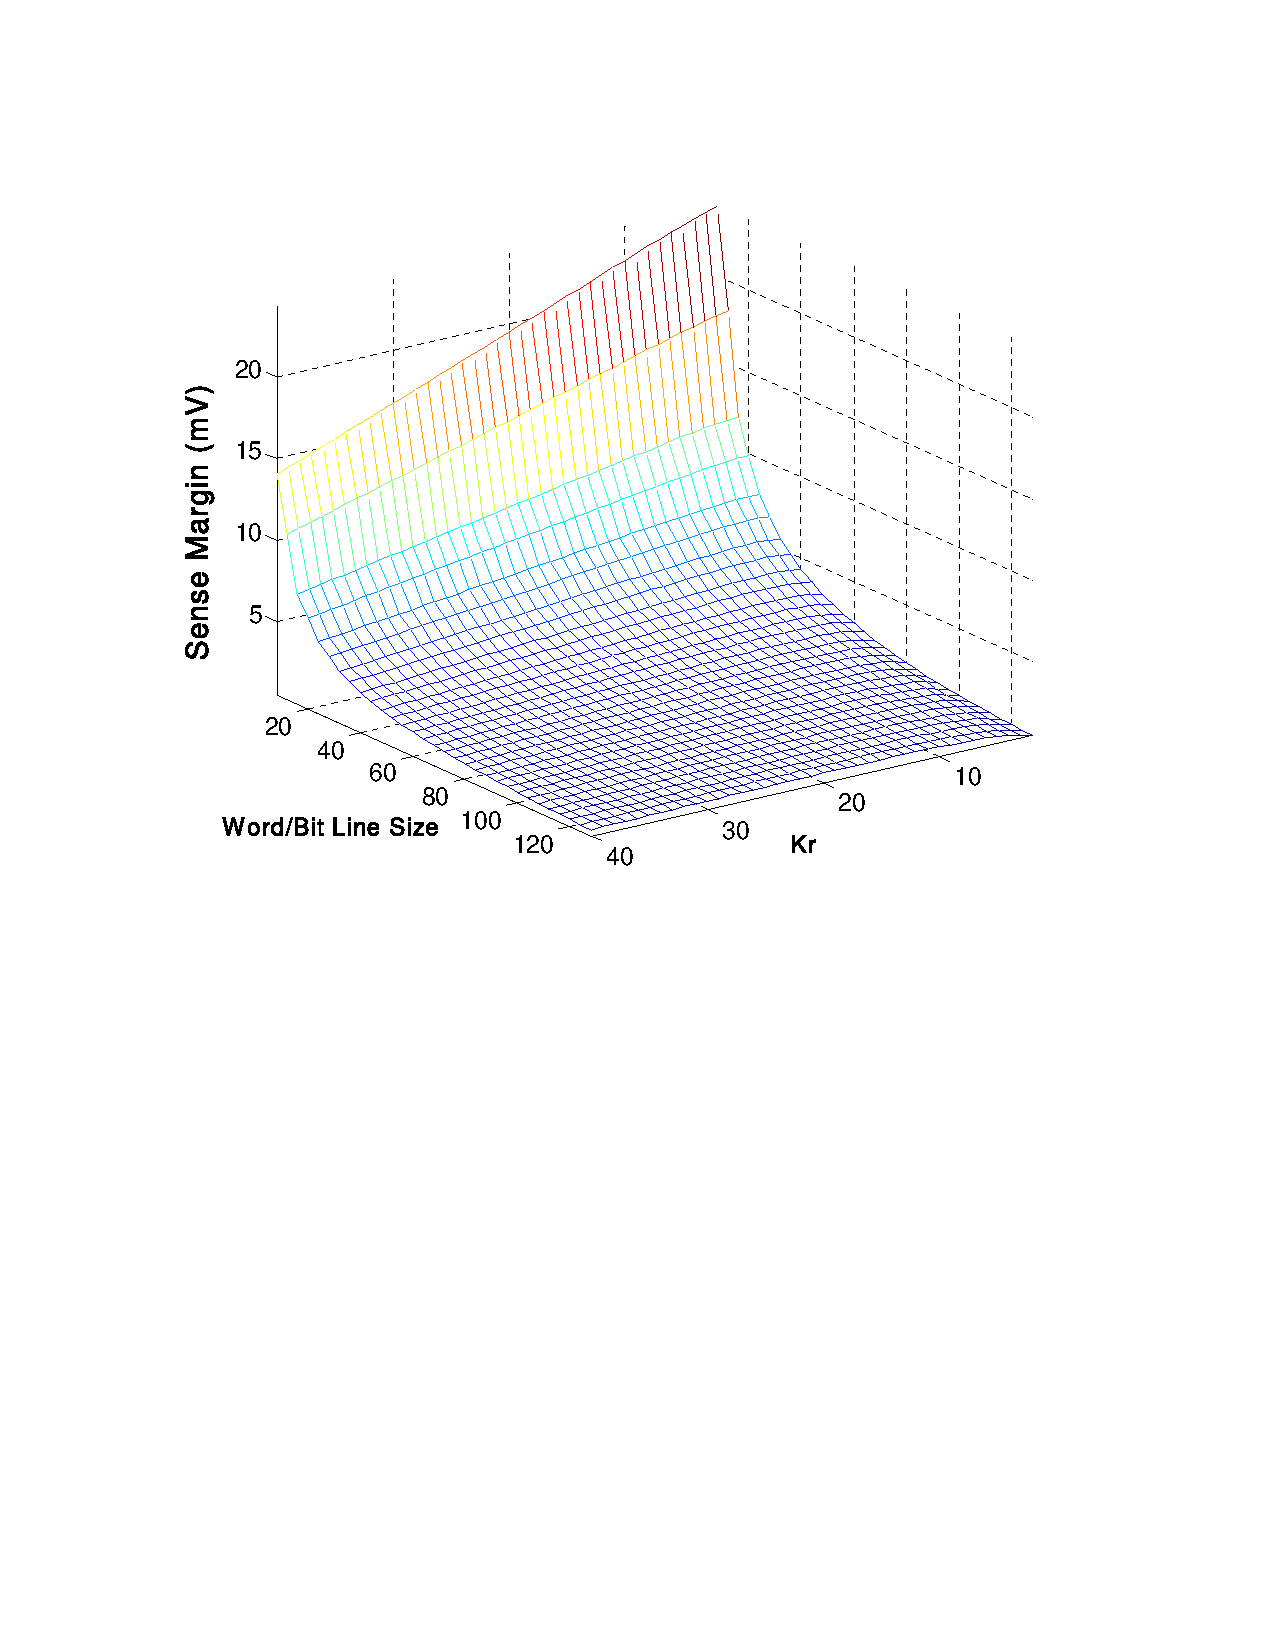
\includegraphics[width=0.45\textwidth]{./figures/margin.pdf}
%  \caption{The}\label{fig:margin}
%\end{figure}
%
%\begin{figure}%[!t]
%\centering
%  % Requires \usepackage{graphicx}
%  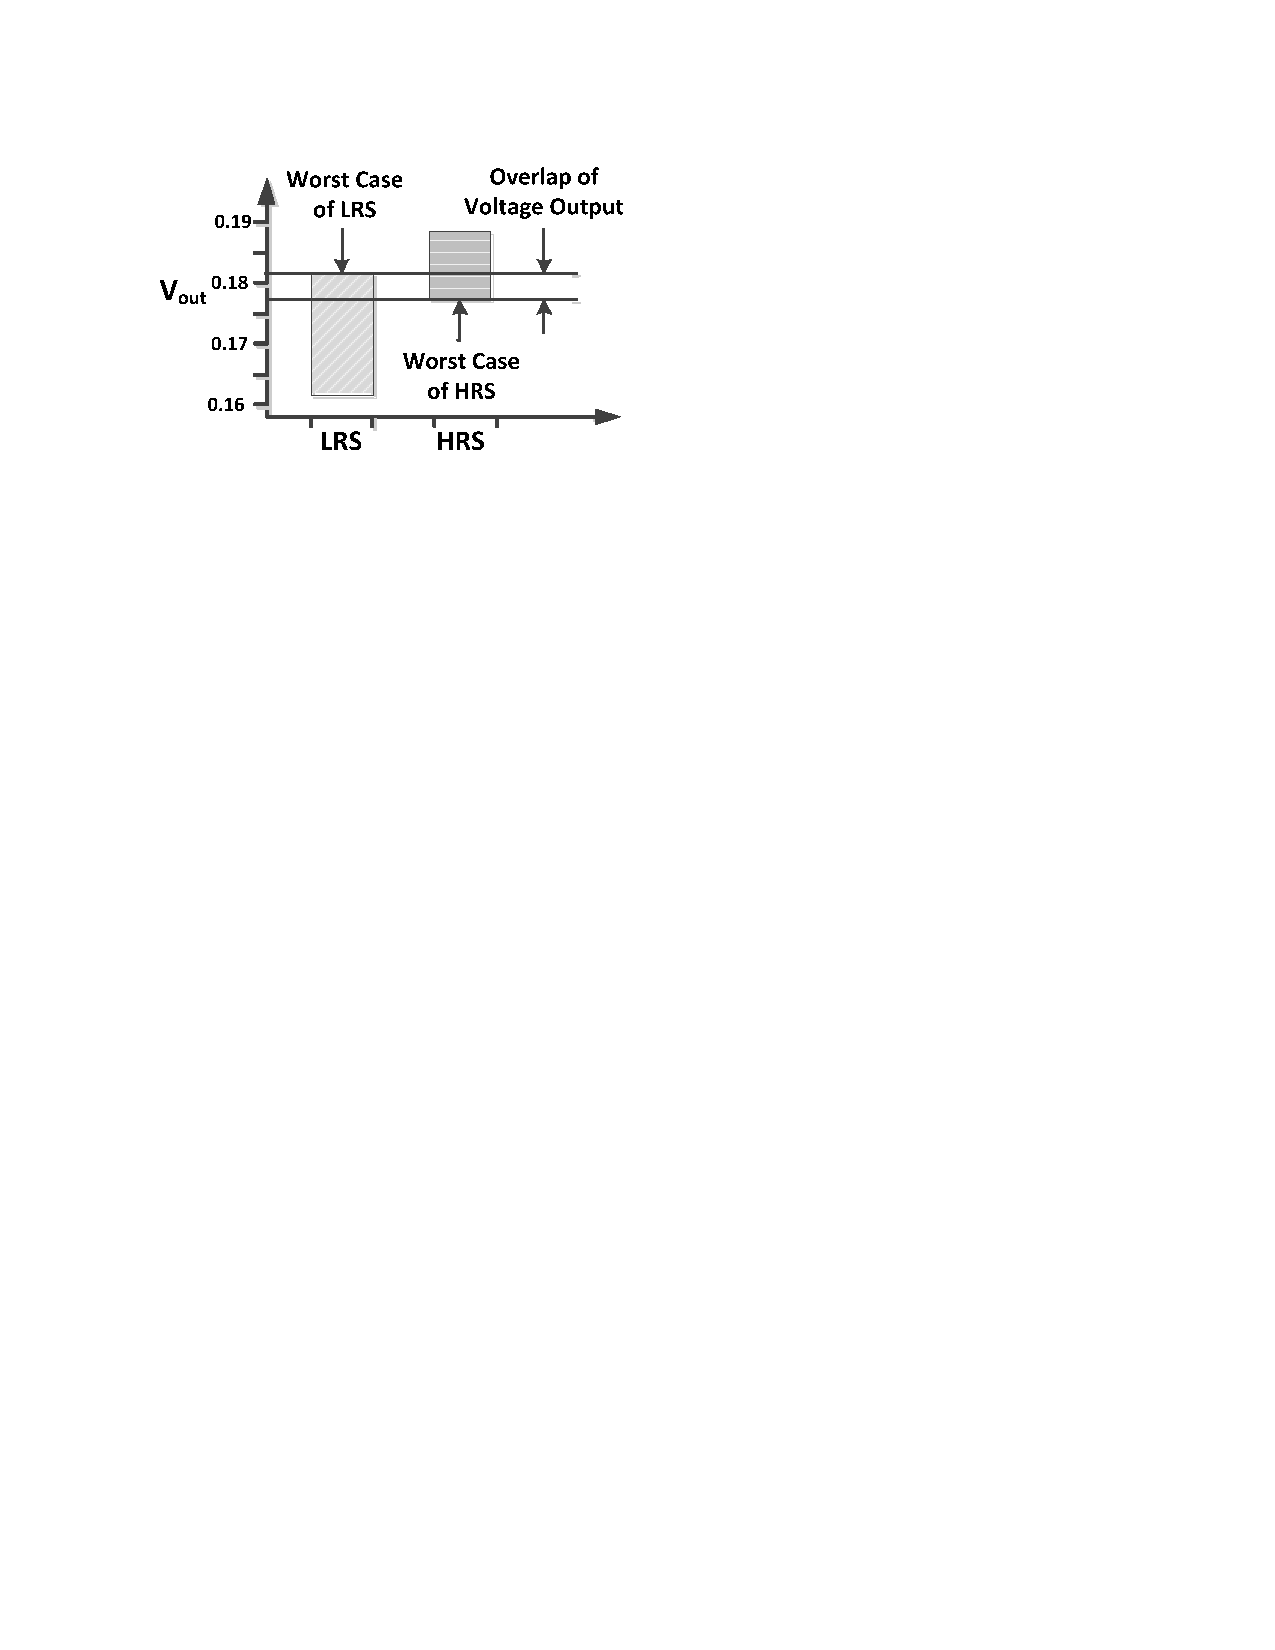
\includegraphics[width=0.4\textwidth]{./figures/overlap.pdf}\\
%  \caption{The}\label{fig:overlap}
%\end{figure}

%
%\begin{figure}%[!t]
%\centering
%  % Requires \usepackage{graphicx}
%  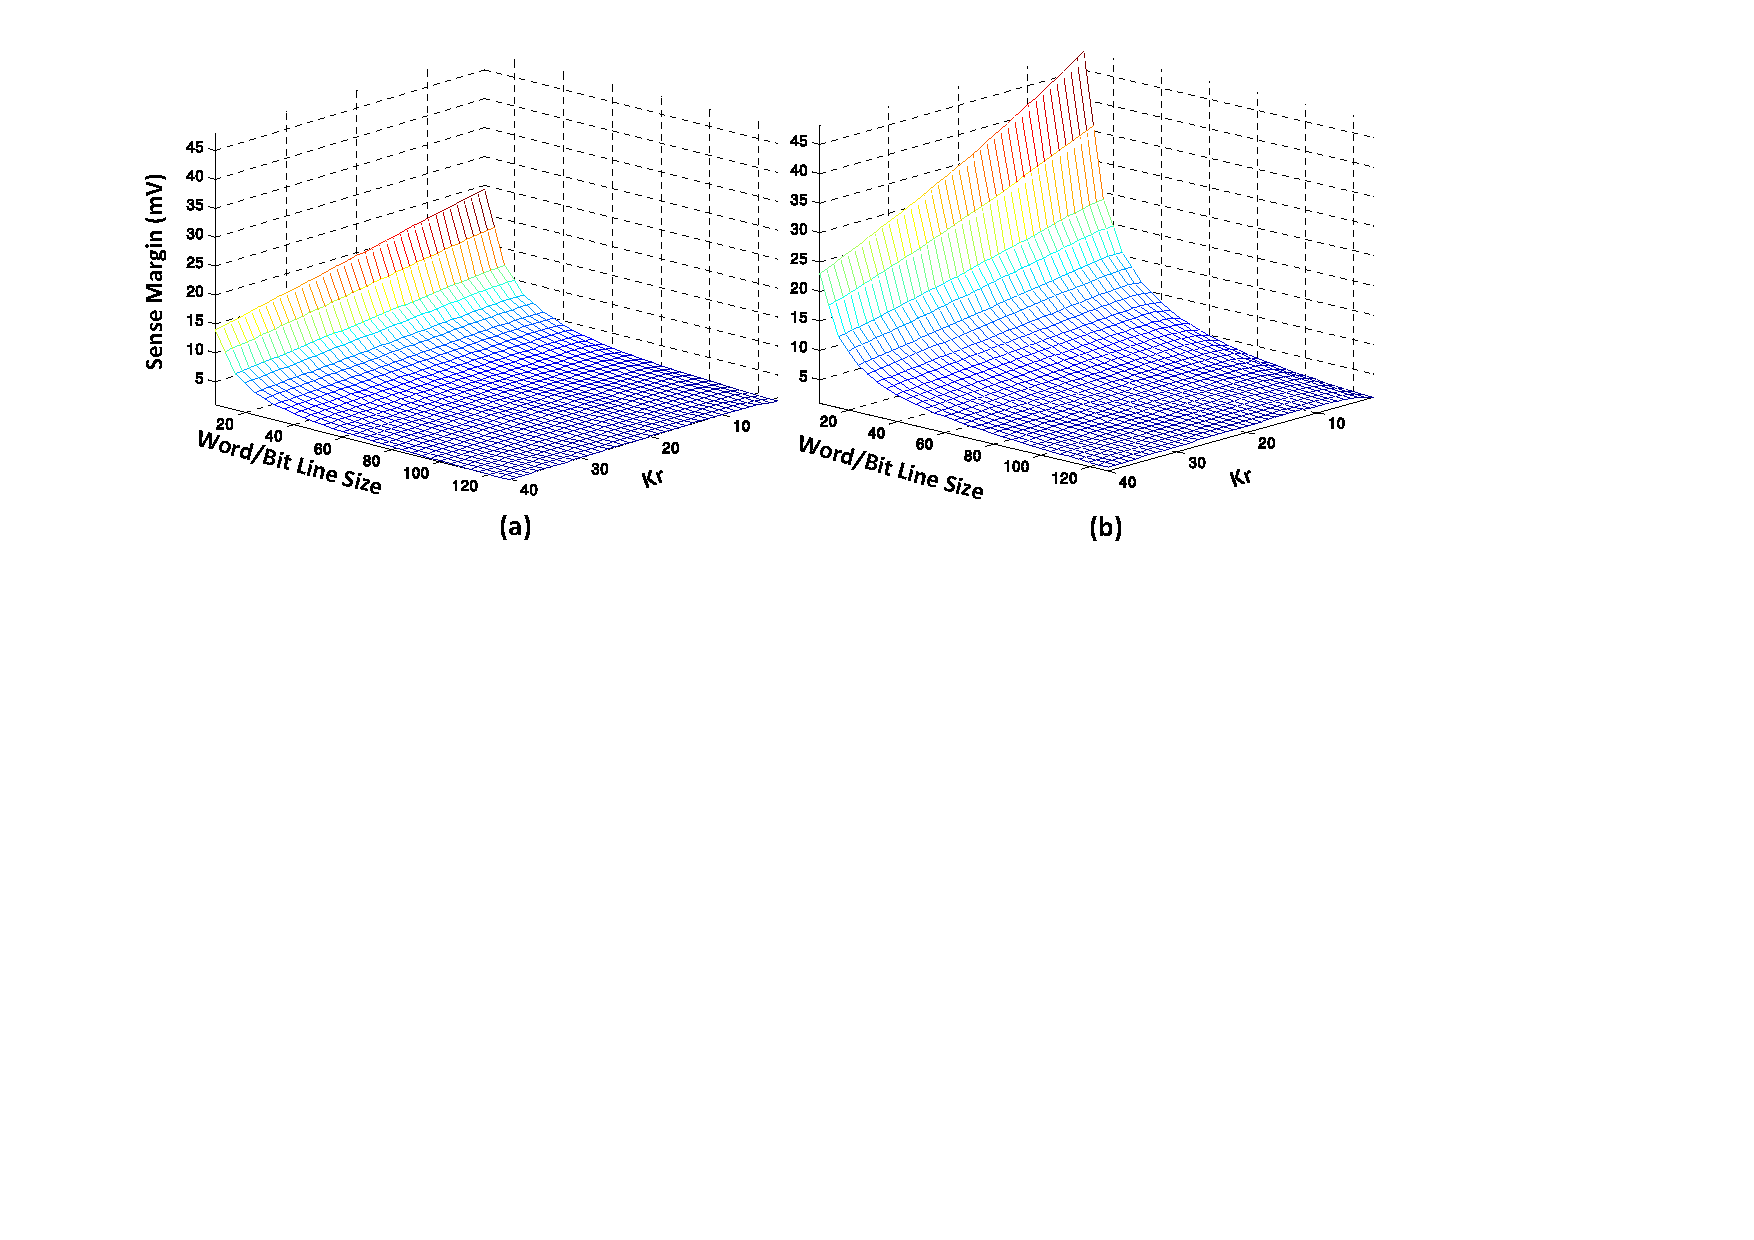
\includegraphics[width=0.5\textwidth]{./figures/sense_margin21}\\
%  \caption{The}\label{fig:sense_margin}
%\end{figure}

\begin{figure}%[!t]
\centering
  % Requires \usepackage{graphicx}
  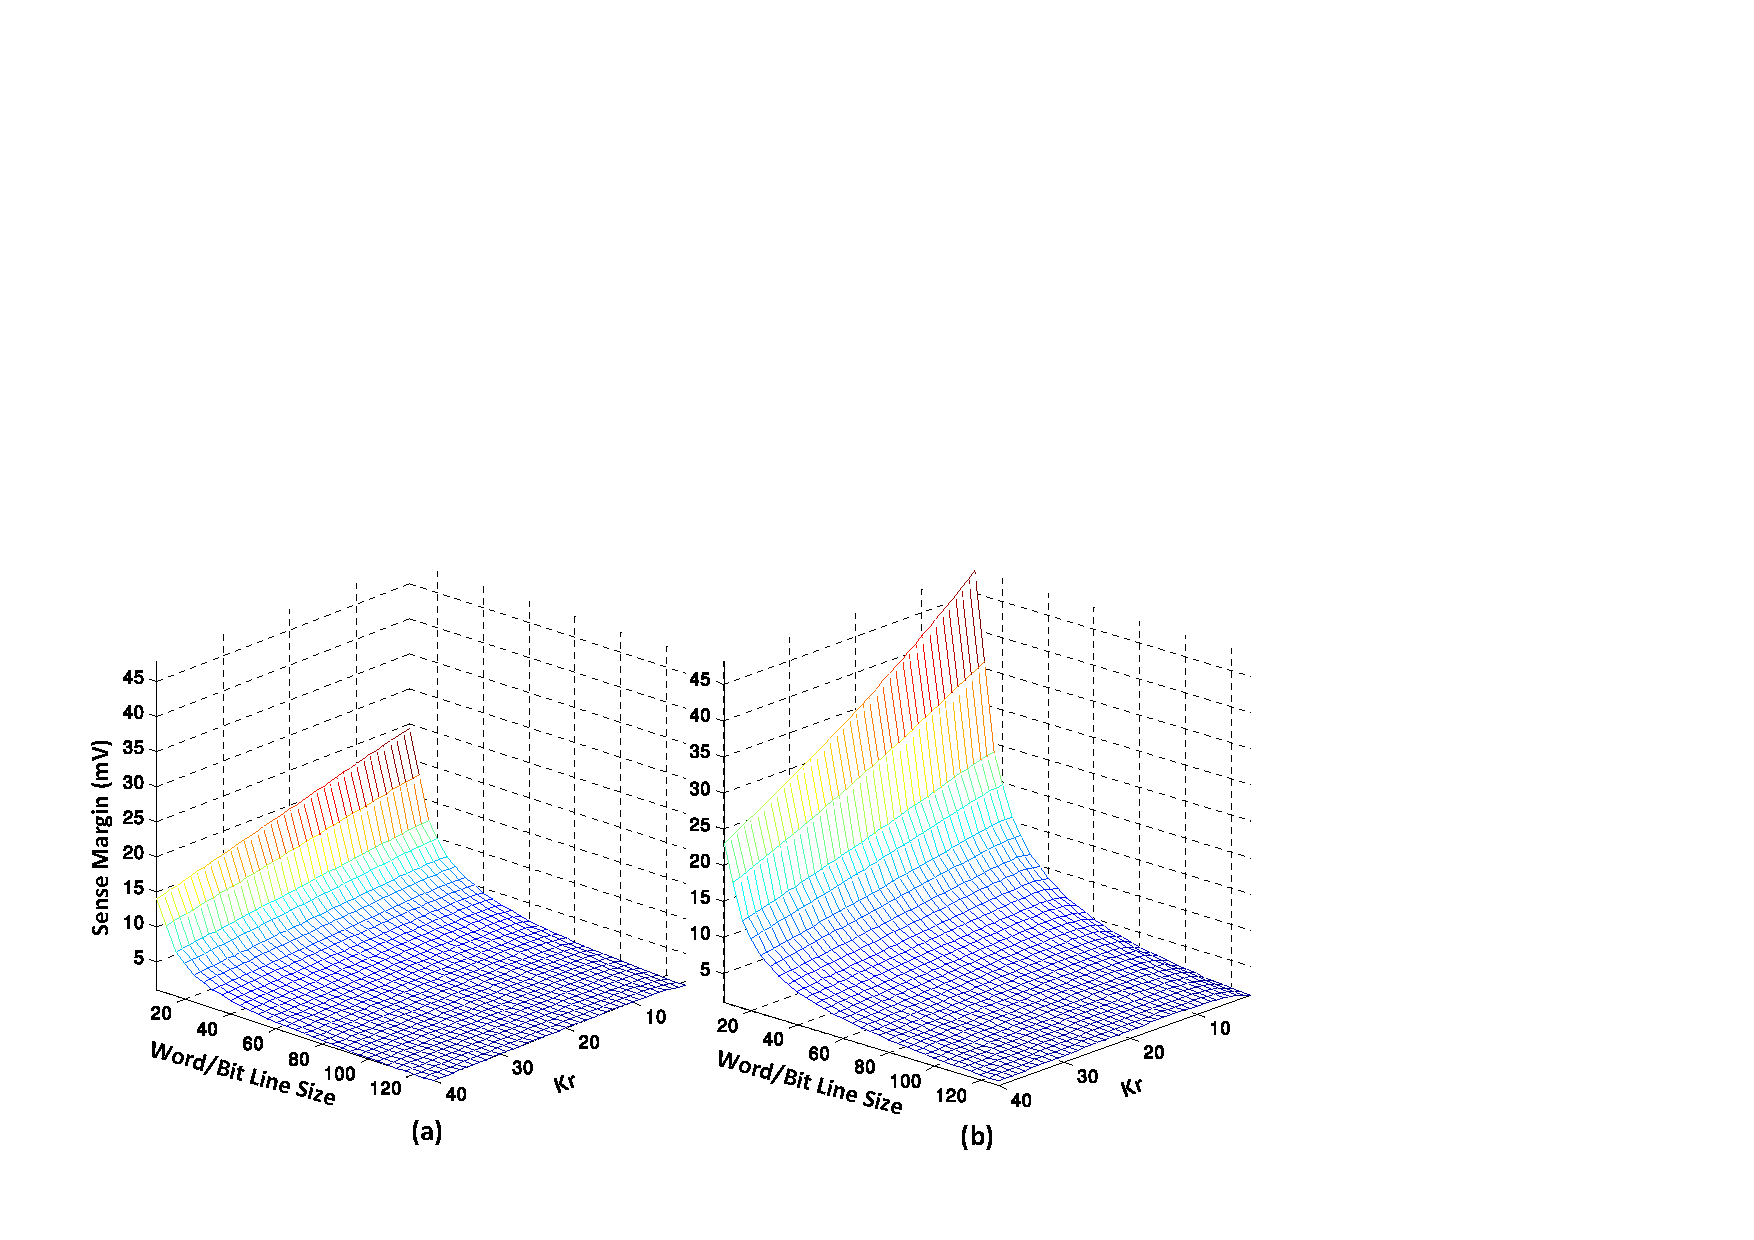
\includegraphics[width=0.5\textwidth]{./figures/sense_margin2}\\
  \caption{The}\label{fig:sense_margin}
\end{figure}
\subsection{Discussion on Non-linearity of the ReRAM}
An
